\documentclass[12pt]{article}
\usepackage{setspace}
\usepackage{amsmath,amsfonts,amssymb,graphicx,setspace,authblk}
\usepackage{titlesec,blkarray, bm} 
\usepackage{float,afterpage}
\usepackage[running,mathlines]{lineno}
\usepackage[vmargin=1in,hmargin=1in]{geometry}
\usepackage[authoryear,sort]{natbib}
\usepackage[dvipsnames]{xcolor}
\usepackage{hyperref}
\doublespacing
\usepackage{enumitem}
\setlist{topsep=.125em,itemsep=-0.15em,leftmargin=0.75cm}
\setlength{\parindent}{0.35in}

\usepackage[sc]{mathpazo} %Like Palatino with extensive math support

% Coloring of R code listings
\usepackage[formats]{listings}
\usepackage{color}
\definecolor{mygreen}{rgb}{0.1,0.5,0.1}
\definecolor{mygray}{rgb}{0.5,0.5,0.5}
\definecolor{mymauve}{rgb}{0.58,0,0.82}
\definecolor{mygrey}{rgb}{0.3,0.3,0.1}
\lstset{
language=R,
otherkeywords={data.frame},
basicstyle=\normalsize\ttfamily, 
commentstyle=\normalsize\ttfamily,
keywordstyle=\normalsize\ttfamily,
stringstyle=\color{mymauve}, 
commentstyle=\color{mygreen},
keywordstyle=\color{blue},
showstringspaces=false, xleftmargin=2.5ex,
columns=flexible,
literate={~}{{$\sim \; \; $}}1,
alsodigit={\.,\_},
deletekeywords={on,by,data,R,Q,mean,var,sd,log,family,na,options,q,weights,effects,matrix,nrow,ncol,wt,fix,distance},
}
\lstset{escapeinside={(*}{*)}} 

\lstdefineformat{Rpretty}{
	; = \space,
	\, = [\ \,\]]\string\space,
	<- = [\ ]\space\string\space,
	\= = [\ ]\space\string\space}


\usepackage{lineno}
\renewcommand{\refname}{Literature Cited}
\renewcommand{\floatpagefraction}{0.98}
\renewcommand{\topfraction}{0.99}
\renewcommand{\textfraction}{0.05}

\clubpenalty = 10000
\widowpenalty = 10000

\sloppy 

\usepackage{ifpdf}
\ifpdf
\DeclareGraphicsExtensions{.pdf,.png,.jpg}
\usepackage{epstopdf}
\else
\DeclareGraphicsExtensions{.eps}
\fi

\DeclareMathOperator{\Ex}{\mathbb{E}}
\DeclareMathOperator{\var}{\textit{Var}}
\DeclareMathOperator{\cov}{\textit{Cov}}



%%%%%%%%% Macros to simplify using our notation 

\newcommand{\s}[1]{{#1}^{\#}}
\newcommand{\f}[1]{{#1}^{\flat}}
\newcommand{\sr}[1]{{#1}^{*}}
\newcommand{\br}[1]{\langle {#1} \rangle} 
\newcommand{\bs}{\backslash} 
\def\alphat{\widetilde{\alpha}}
\newcommand{\half}{\frac{1}{2}}

% commands for commenting
\newcommand{\tom}[2]{{\color{red}{#1}}\footnote{\textit{\color{red}{#2}}}}
\newcommand{\steve}[2]{{\color{blue}{#1}}\footnote{\textit{\color{blue}{#2}}}}

% Define Box environment for numbered boxes. 
\newcounter{box}
\newcommand{\boxnumber}{\addtocounter{box}{1} \thebox \thinspace}

\floatstyle{boxed}
\newfloat{Box}{tbph}{box}

%%%%%%%%%%%%%%%%%%%%%%%%%%%%%%%%%%%%%%%%%%%%% 
%%% Just for commenting
%%%%%%%%%%%%%%%%%%%%%%%%%%%%%%%%%%%%%%%%%%%%
\usepackage[dvipsnames]{xcolor}
\newcommand{\comment}{\textcolor{blue}}
\newcommand{\new}{\textcolor{red}}

\newcommand{\be}{\begin{equation}}
\newcommand{\ee}{\end{equation}}

\newcommand{\red}{\textcolor{red}}

\title{My, how you've grown: a practical guide to modeling size transitions for Integral Projection Model (IPM) applications}

\author[a]{Tom E.X. Miller\thanks{Corresponding author. Department of BioSciences, Rice University,
Houston, TX 77005-1827. Email: tom.miller@rice.edu Phone: 713-348-4218}}
\author[b]{Stephen P. Ellner}
\affil[a]{Department of BioSciences, Rice University, Houston, TX } 
\affil[b]{Department of Ecology and Evolutionary Biology, Cornell University, Ithaca, New York} 
\date{}
\renewcommand\Authands{ and }

\sloppy


\begin{document}

\renewcommand{\baselinestretch}{1.25} 
\maketitle

\bigskip 
%45 character limit on running head
\noindent\textbf{Running header:} Better growth modeling for IPMs

\newpage
\linenumbers
%%%%%%%%%%%%%%%%%%%%%%%%%%%%%%%%%%%%%%%%%%%%%%%%%%%%%%%%%%%%%%%%%%%%%%
\spacing{1.25} 
%350 word limit on abstract, must be numbered 1-4
\section*{Abstract} 
\begin{enumerate}
	\item 
	\item 
	\item 
	\item 
\end{enumerate}

%alphabetical order not exceeding eight words or short phrases
\section*{Keywords}

\newpage
\section*{Introduction}

Structured demographic models -- matrix and integral projection models (MPMs and IPMs) -- are powerful tools for data-driven modeling of population dynamics and viability that are widely used in basic and applied settings. 
In contrast to MPMs for populations with discrete structure (life stage, age class, etc.), IPMs \citep{easterling2000size} readily accommodate populations structured by continuous state variables, most commonly size. 
A related innovation of the IPM framework is its emphasis on regression-based modeling for parameter estimation, which carries important advantages for making the most of hard-won data \citep{ellner2022critical}.  

A standard workflow allows ecologists to assemble an IPM from data using familiar statistical tools to describe growth, survival, reprduction, and other demographic transitions as functions of size \citep{Coulson:2012fk,ellner-etal-2016}. 
The relative ease of the regression-based approach, accommodating multiple covariates (e.g., environmental factors, experimental treatments) and complex variance structures (e.g., random effects, correlated errors), has facilitated a growing body of IPM literature that examines how biotic or abiotic factors affect population dynamics \citep[e.g.,][]{schultz2017native,ozgul2010coupled,louthan2022climate} and explores the consequences of demographic heterogeneity associated with spatial, temporal, and individual variation \citep[e.g.,][]{crone2016contrasting,compagnoni2016effect,plard2018sex}. 
The vital rate regressions (or ``sub-models'') are the bridge between the individual-level data and the population-level model and its predictions; it is important to get them right.

Compared to other vital rates, growth is special. 
The regression sub-models for survival and reproduction provide the expected values of those rates as functions of size (we use ``size'' as the name for whatever continuous variable defines the population structure, which could instead be immune competence, mother's weight, etc.).   
However, for modeling growth, the full probability distribution of subsequent size, conditioned on initial size, must be defined. 
This distribution defines the growth `kernel' $G(z',z)$ that gives the probability density of any future size $z'$ at time $t+1$ conditional on current size $z$ at time $t$. 
Whenever survival and reproduction are size-dependent, the entire distribution of size transitions can strongly influence IPM predictions because this distribution governs how frequently size changes are much greater or much lower than average. 

The original template for modeling size transitions in IPMs was provided by Easterling et al. \citeyear{easterling2000size}. 
They first tried simple linear regression, assuming normally distributed size changes with constant variance. 
Because the residuals from this regression exhibited non-constant variance, they used a two-step approach that estimated the size-dependence in the growth variance (better options soon became available, such as the \texttt{lme} function in R). 
However, even after accounting for non-constant variance, growth data may still deviate from the assumption that size transitions are normally distributed.  
Size transitions are often skewed such that large decreases are more common than large increases \citep{peterson2019improving,salguero2010keeping}, or vice versa \citep{stubberud2019effects}.
Size transitions may also exhibit excess kurtosis (`fat tails'), where extreme growth or shrinkage is more common than predicted by the tails of the normal distribution \citep{herault2011functional}. 

The observation that the normal distribution may poorly describe size transitions in real organisms has been made before,  
and several studies have emphasized that alternative distributions should be explored \citep{easterling2000size,peterson2019improving,rees2014building,williams2012avoiding}. 
Yet, default use of Gaussian growth distributions (often with non-constant variance) remains the standard practice. 
\tom{An ISI Web of Knowledge search on the terms `integral projection model ecology' (DATE) returned \# IPM studies published in the past decade (2010--2020), \# of which assumed a Gaussian growth kernel.}{I still intend to do this! But it's a rabbit hole I have not gone down yet.}
The general state-of-the-art in the literature appears to remain where it was 20 or so years ago, using the default model without pausing to examine critically whether or not it actually provides a good description of the data. 
We are guilty of this, ourselves. 

The persistence of Gaussian growth modeling is understandable. 
There is a long tradition of statistical modeling built on the assumption of normally distributed residuals with constant variance.
Popular software pacakges such as lme4 \citep{bates2007lme4} and MCMCglmm \citep{hadfield2010mcmc} make it easy to fit growth models with potentially complex fixed- and random-effect structures, but the possible distributions of continuous responses are limited, and default to Gaussian.
Abandoning these convenient tools for the sake of more flexible growth modeling means, it may seem, sacrificing the flexibility to rigorously model diverse and potentially complex sources of variation in growth, some of which may be the motivation driving the study in the first place.

The question we address here is: how can ecologists escape the apparent trade-off between realistically capturing the variance, skew, and kurtosis of size transition data on the one hand, and flexibly including the multiple covariates and random effects that often have substantial impacts on demographic rates.  
In this article, we offer an answer. 

Our goal here is to present and illustrate a general `recipe' that moves growth modeling past the standards set over 20 years ago.
Like any recipe, users may need to make substitutions or add ingredients to suit their situation. 
Our approach emphasizes graphical diagnostics for developing and evaluating growth models, rather than a process centered on statistical model selection. 
Through a set of empirical case studies we demonstrate how a simple workflow, using tools that were nonexistent or not readily available when IPMs first came into use, makes it straightforward and relatively easy to identify when the default model is a poor fit to the data, and to then choose and fit a substantially better growth model that is no harder to use in practice. 
\tom{We illustrate our approach by revisiting four of our own, mostly published IPM analyses that assumed Gaussian growth.}{Need to commit to case study choices - Steve wanted to include corals for contrast with Peterson et al.} 
In each case, the Gaussian assumption does not stand up to close scrutiny. 
We illustrate how we could have done better, and the consequences of ``doing better'' 
for our ecological inferences. 
All of our analyses may be reproduced from code and data that are publicly available (see Data accessibility statement).

\section*{A general workflow for better growth modeling}
The modeling workflow that we suggest runs as follows (Fig. \ref{fig:workflow}):
\begin{enumerate}[label=\arabic*., listparindent=1.5em]
\item \textit{Fit a ``pilot'' model or models assuming a Gaussian distribution but allowing for non-constant variance.}
\\ 
This step is familiar to most IPM users, as it is the start and end of the traditional workflow. 
A well-fitted Gaussian model accurately describes the mean and variance of future size conditional on current size and possibly on other measured covariates or random effects. 
This step may include model selection to identify which treatment effects or environmental drivers affect the mean and/or variance of future size. 
Non-constant variance is often fitted in a two-stage process, first fitting mean growth assuming constant variance, then doing a regression relating the squared residuals from the initial fit to the fitted mean. 
It is sometimes better to fit size-dependence in the mean and variance simultaneously, as can be done with the R packages \textbf{mgcv} and \textbf{nmle}, because incorrectly assuming constant variance can affect the outcome of model selection for the mean. 
One-step fitting is straightforward for simple models in which initial size is the only factor that can influence growth variance. 
However, the two-step process fitting residuals to the fitted value (expected future size) may be convenient when there are multiple fixed and random effects, all of which may contribute to non-constant variance, since the expected value implicitly accounts for all of them. 
We illustrate both one-step and two-step approaches in the examples below. 

Allowing non-constant variance means that it is not necessary to transform the data in a way that stabilizes the growth variance. 
Transformation remains an option when it does not create new problems (see Discussion), and it may have advantages besides variance stabilization. %beta regression
In particular log-transformation is often appropriate for size data \citep{ellner-etal-2016}, and it helps avoid eviction at small sizes. 

\item \textit{Use statistical and graphical diagnostics to identify if and how the standardized residuals deviate from Gaussian, and to identify a more appropriate distribution.}
\\
If the Gaussian pilot model is valid, the set of standardized residuals (standardized by the standard deviation) should be Gaussian with mean zero and unit variance, with no skew or excess kurtosis. 
This criterion provides a straightforward test for whether to accept a Gaussian growth model or explore alternatives. 
If the standardized residuals are satisfactorily Gaussian, skip to the final step of the workflow. 

There are many ways that growth data may deviate from Gaussian, and the nature of those deviations can guide the search for a better distribution. 
Frequentist tests such as the D'Agostino test of skewness \citep{d1970transformation} and the Anscombe-Glynn test of kurtosis \citep{anscombe1983distribution} could be used to diagnose whether the aggregate distribution of standardized residuals deviates from normality (R package \textbf{moments} \citep{komsta2015moments}). 
However, the aggregate distribution of standardized residuals may be misleading if properties such as skew and kurtosis vary with size. 
For example, a change in the direction of skewness from small to large sizes would require a distribution flexible enough to accommodate both positive and negative skew, such as the skewed normal or Johnson $S_{U}$ distributions. 
Alternatively, growth data may lack skew but may exhibit leptokurtosis (in which case the $t$ distribution may be a good choice) or may shift from platykurtosis to leptokurtosis depending on initial size (in which case the power exponential distribution may be a good choice). 
It is therefore essential to visualize trends in distribution properties with respect to size, either initial size (for simple models with only size-dependence) or expected future size (for models with multiple fixed effects). 
In the case studies below, we rely on quantile regression of the standardized residuals to visualize skew and kurtosis as continuous functions of size or expected value. 
Fig. \ref{fig:workflow} includes guidance on how the skew and kurtosis properties of the standardized residuals suggest options for an appropriate growth distribution. 
In our case studies we take advantage of the many distributions provided in the \textbf{gamlss} R package \citep{stasinopoulos2007generalized}, but any other distributions with the necessary properties can be used.  

\item \textit{Refit the growth model using the chosen distribution.}
\\
In models with multiple covariates and/or random effects, each potentially affecting several distribution parameters (location, scale, skew, kurtosis) in
different ways, ``refit the model'' could entail a massive model selection process to identify the ``right'' or ``best'' non-Gaussian model. 
And with so many options, model uncertainty may be overwhelming and over-fitting becomes a significant risk even if precautions against it are taken. 
We therefore argue for adopting the more modest goal of remedying the apparent defects in the Gaussian model. 
Conveniently, as we demonstrate below, the functional forms for the mean and standard deviation (or location and scale parameters) could be carried over from the pilot Gaussian model into a non-Gaussian distribution, leaving skew and kurtosis as the targets for improvement. 
This step exploits the fact that parameter estimation from a Gaussian model is generally robust to deviations from normality \citep{schielzeth2020robustness}, meaning that the mean of the Gaussian model is probably a good proxy for the mean of the non-Gaussian model (and in case it is not, the next step in the workflow would catch that). 
The functional forms for skew and kurtosis of the non-Gaussian model can be guided by the qualitative features of the graphical diagnostics (e.g., skewness switches from positive to negative with size). 
%When there are other covariates or random effects, the GLM-like alternative of making distribution parameters a function of the location parameter (the ``linear predictor'') sould also be considered. 
%How fitting is accomplished depends on features of the model, in particular whether or not it includes random effects. 

\item \textit{Test the final model through graphical diagnostics comparing simulated and real growth data.} 
\\
A good model will generate simulated data that look like the real data.  
Again, it is important to inspect the properties of simulated data conditional on present size or expected future size, rather than examining the entire distribution.   
We provide examples below of informative comparisons between simulated and real data, based mainly on quantiles. 
If the simulated data do not correspond well with real data, alternative (possibly more flexible) growth distributions should be explored, or more complex
functions relating distribution parameters to current size and other covariates. 
However, we again caution against launching a full-blown model selection exercise. 
Instead, possible alternative models could be chosen primarily to remedy observable discrepancies between the real and simulated size transition data, and at most slightly modified based on final diagnostic and statistical tests.

\end{enumerate}

\begin{figure}
\centering
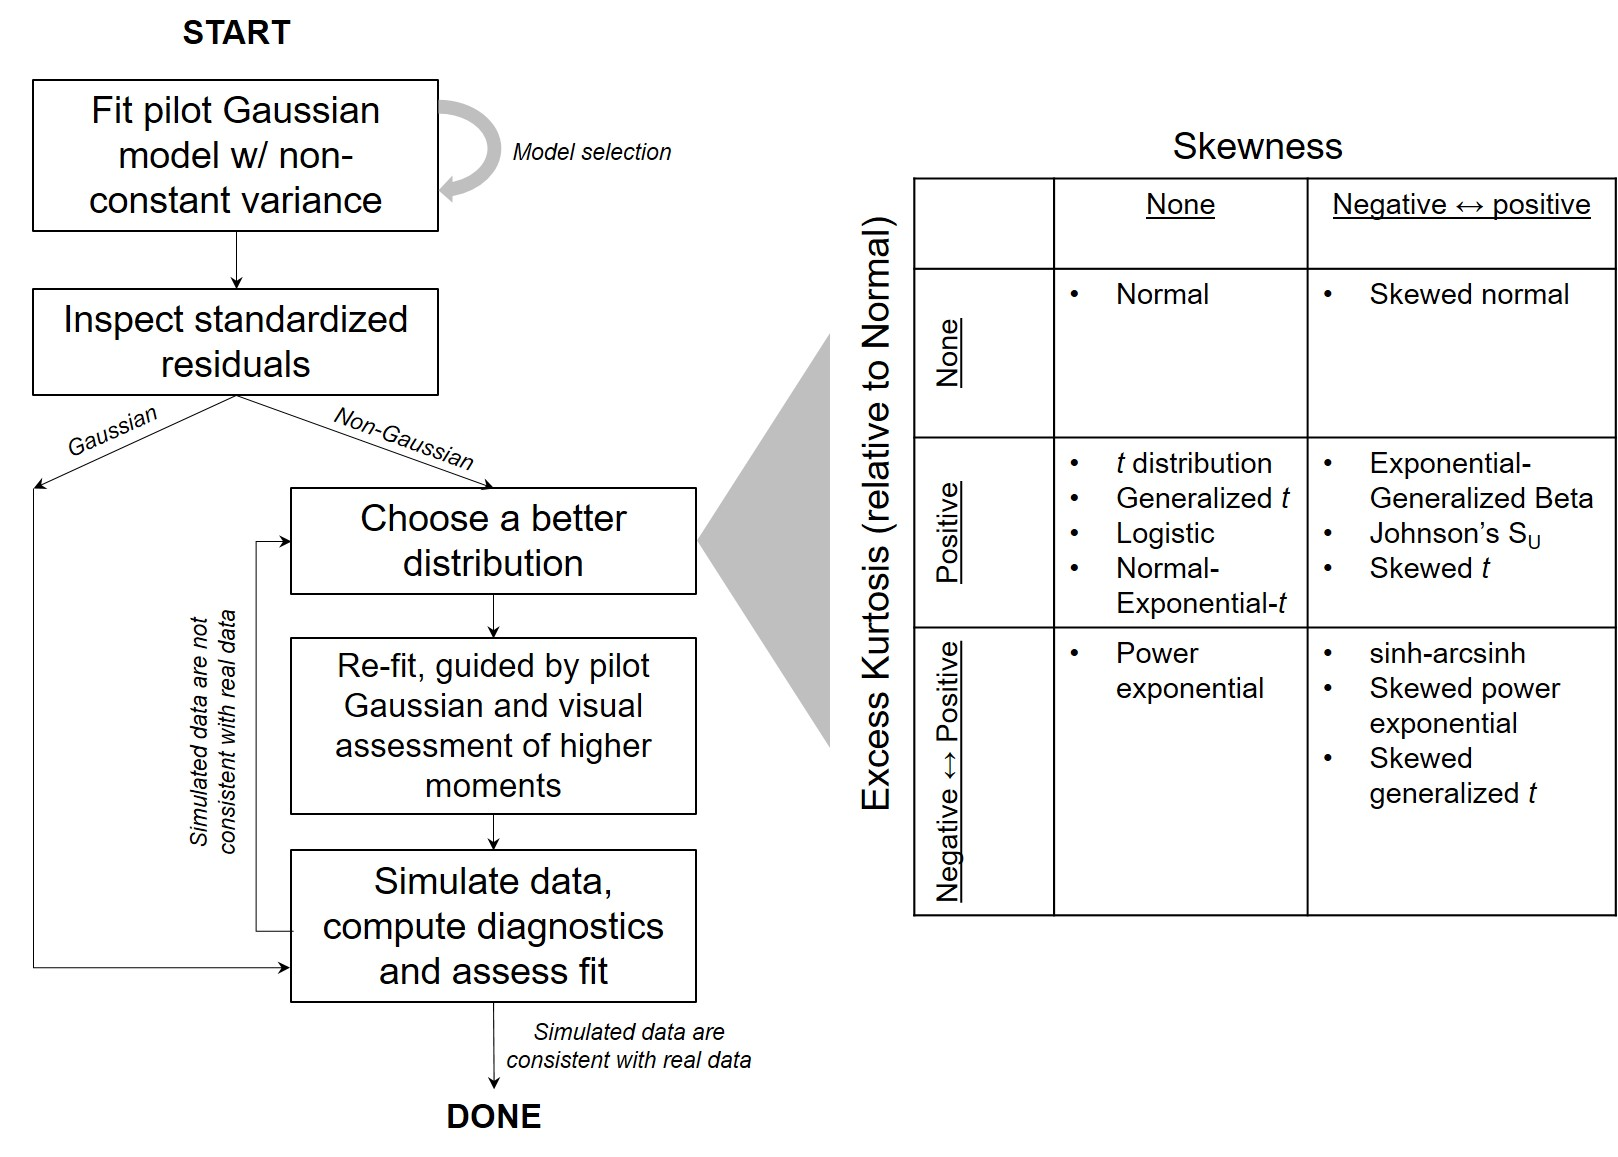
\includegraphics[width=\textwidth]{figures/workflow}
\caption{General workflow of recommendations for IPM growth modeling (left) and guide to common non-Gaussian distributions of size $x$ for $x \in \mathbb{R}$ that can accommodate different combinations of skewness and kurtosis (right). 
All of these distributions (often including multiple versions or parameterizations of each) are available in the package \textbf{gamlss.dist}, 
except for the skewed generalized $t$, which is available in the package \textbf{sgt} \citep{davis-2015}.}
%\textbf{actuar} \citep{dutang2008actuar}.
\label{fig:workflow}
\end{figure} 

\section*{How should skewness and kurtosis be measured?}
``Improvement'' of a Gaussian model will always involve scrutiny of skewness and kurtosis, so measurement of these properties warrants some attention. 
The standard measures of skewness and kurtosis (tail thickness) are based on the third and fourth central moments, respectively, of the distribution: 
\be
\mbox{Skewness} = \frac{m_3}{\sigma^3}, \quad \mbox{Excess kurtosis} = \frac{m_4}{\sigma^4}-3
\ee
where $m_k = \mathbb{E}(X - \bar{X})^k$ is the $k^{th}$ central moment of a random quantity $X$ 
and $\sigma^2$ is the variance (second central moment). 
A Gaussian distribution has zero skewness and zero excess kurtosis. 

The standard measures are easy to calculate but their use for choosing and evaluating growth models is hindered by their poor sampling properties. 
Because empirical estimates involve high powers of data values, it only takes a 
a few outliers to produce a very inaccurate estimate. 
Figure \ref{fig:NPmoments} shows a simulated example, where the underlying ``data'' are a sample of size 200 from a $t$ distribution with 8 degrees of freedom; the true skew is 0, and the true excess kurtosis is 1.5. 
The distance between the largest and smallest estimates (indicated by the dotted red vertical lines), relative to the distance between the 5th and 95th percentiles, shows the broad extent of extreme values that can occur even with a good size sample, especially for kurtosis. 

\begin{figure}[tbp]
\centering
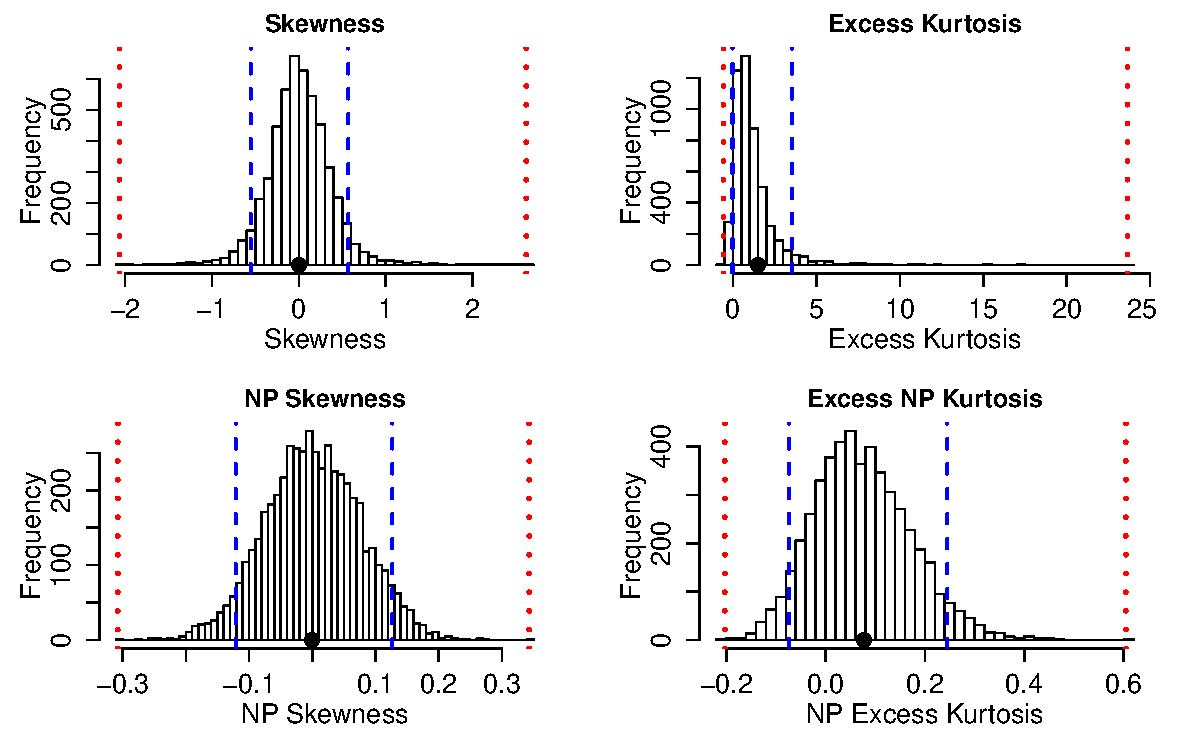
\includegraphics[width=\textwidth]{figures/NPmoments.pdf}
\caption{Histograms of skewness and kurtosis estimates using moment-based definitions, compared with the nonparametric measures. 
Histograms are based on 5000 replicate draws of a sample of 200 independent values fron a $t$ distribution with 8 degrees of freedom. 
Dotted red vertical lines mark the minimum and maximum of sample estimates, and dashed blue lines show the 5th and 95th percentiles. 
The true value is indicated by a black dot on the $x$-axis.
Figure drawn by script \texttt{NPmoments.R}}
\label{fig:NPmoments}
\end{figure} 

We therefore use ``nonparametric'' (NP) measures of skew and kurtosis that are based on quantiles and thus less sensitive to a few extreme data values. 
Let $q_\alpha$ denote the $\alpha$ quantile of a distribution or sample (e.g., $q_{0.05}$ is the 5th percentile). 
For any $0 < \alpha < 0.5$, a quantile-based measure of skewness is given by \citep{mcgillivray-1986}
\be
\mbox{NP Skewness} = \frac{q_\alpha + q_{1-\alpha} - 2 q_{0.5}}{q_{1-\alpha} - q_\alpha}.
\ee
NP Skewness is a measure of asymmetry between the tails of the distribution above and below the median. 
The size of the upper tail can be measured (for any $0 < \alpha < 0.5$) by $\tau_U = q_{1-\alpha} - q_{0.5}$; for $\alpha=0.05$ this is the difference
between the 95th percentile and the median. 
The lower tail size is $\tau_L = q_{0.5} - q_\alpha$. The definition above is equivalent to  
\be
\mbox{NP Skewness} = \frac{\tau_U - \tau_L}{(\tau_U + \tau_L)}.
\label{eqn:NPskew}
\ee
So an NP Skewness of $\pm 0.2$ says that the difference in tail sizes is 20\% of their total. 
The range of possible values is -1 to 1. Both $\alpha=0.25$ (sometimes called ``Kelly's skewness'') and $\alpha=0.1$ (``Bowley's skewness'') are common choices. 
We used $\alpha=0.1$, unless otherwise stated.  
 
An analogous quantile-based measure of kurtosis \citep{jones-etal-1994} is 
\be
\mbox{NP Kurtosis}  = \frac{q_{1-\alpha} - q_{\alpha}}{q_{0.75} - q_{0.25}}.
\label{eqn:NPkurt}
\ee
For $\alpha=0.05$, NP Kurtosis is the difference between the 95th and 5th percentiles, relative to the interquartile range. 
To facilitate interpretation, we scale NP Kurtosis relative to its value for Gaussian distribution, and subtract 1. 
We call this ``NP Excess Kurtosis''. 
The value for a Gaussian distribution is zero. 
A value of 0.2 means that the tails are (on average) 20\% heavier than those of a Gaussian with the same interquartile range, and a value of -0.2 means that the tails are (on average) 20\% lighter than a Gaussian with the same interquartile range. 
We calculate NP Kurtosis using $\alpha=0.05$ unless otherwise stated, to focus on the tail edges, but again this is somewhat arbitrary. 

Figure \ref{fig:NPmoments}C,D illustrate how, applied to exactly the same simulated samples, the non-parametric measures of skewness and kurtosis produce a smaller fraction of highly inaccurate estimates caused by a few extreme values in the sample. 
But also note that, in contrast to the moment-based measures, numerically small values of the NP measures (e.g., 0.1 or 0.2) should not be disregarded, because they are both scaled so that a value of 1 indicates extremely large departures from a Gaussian distribution. 

Quantile-based estimation of skewness and kurtosis carries the added value that quantile regression methods may be used to derive these properties of size transitions as continuous functions of initial size or expected future size. 
In the examples below, we use the \textbf{qgam} package to fit smooth additive quantile regression models, which have the flexibility to accommodate non-linear size-dependence in skewness and kurtosis. 
One risk of a gam-based approach is that fitted quantiles may be too ``wiggly'' without constraints on their complexity (in the examples below, we specify $k=4$ to constrain the dimension of the basis function). 
For the gam-averse, other quantile regression models may be equally suitable. 
For consistency with non-parametric skewness and kurtosis, we similarly use quantile-based measures of mean and variance and quantile regression to visualize these as size-dependent. 
Specifically, following \cite{wan2014estimating},
\be
\mbox{NP Mean}  = \frac{q_{0.25} + q_{0.5} + q_{0.75}}{3}
\label{eqn:NPmean}
\ee
and
\be
\mbox{NP SD}  = \frac{q_{0.75} - q_{0.25}}{1.35}.
\label{eqn:NPsd}
\ee
\section{Case study: Sea fan corals, \emph{Gorgonia ventalina}}
We begin with a simple example where current size is the only predictor of future size. 
\cite{bruno-etal-2011} developed an IPM to understand the rise and fall of a fungal pathogen \emph{Aspergillus sydowii} in Caribbean sea fan corals \emph{G. ventalina}. 
The model was based on repeated observations of marked corals in permanent transects at several sites near Akumal, Mexico, recording disease status (infected/uninfected) and the area of uninfected tissue. 
The epidemic peak had passed and disease incidence was already low, so infected fans were relatively infrequent. 
We therefore limit the analysis here to uninfected individuals.
\citet{bruno-etal-2011} found statistically significant year and site effects, but as those explained a very small fraction of the variation in growth increments, they fitted a single growth model to data pooled across years and sites. 
We do the same here. 
The pooled data set consists of 358 observed size transitions. 
The data exhibited size-dependent variance in growth (change in area, $cm^2$), which \cite{bruno-etal-2011} chose to stabilize by transforming size, using the cube-root of total fan area as the size measure (fig. \ref{fig:AkumalPilot}B), and then fitting the standard model with Gaussian growth increments. 
Here we take a different approach, modeling size-dependent variance explicitly rather than trying to transform it away. 

We develop a model using natural log transformation of area. 
With initial size as the only predictor, a simple way to fit a Gaussian model with nonconstant variance is the \texttt{gam} function in \textbf{mgcv} library \citep{wood-2017} using the \texttt{gaulss} family. 
The mean and standard deviation are both fitted as smoothing spline functions of initial size, and the \texttt{predict} function returns the fitted mean and also the inverse of the fitted standard deviations with which we can compute the scaled residuals: 
\begin{lstlisting}
# XH is a data frame holding the data
# logarea.t0, .t1 denote initial and final values of log-transformed area   
fitGAU <- gam(list(logarea.t1~s(logarea.t0),~s(logarea.t0)),
              data=XH, gamma=1.4, family=gaulss())
fitted_all = predict(fitGAU,type="response"); 
fitted_sd = 1/fitted_all[,2]; 
scaledResids = residuals(fitGAU,type=''response'')/fitted_sd;  
\end{lstlisting}
Fig. \ref{fig:coral_diganostics}A shows the log-transformed data and Gaussian model. 
The mean function (solid blue curve) is visually nearly linear, but the fitted nonlinear spline is strongly favored over a linear model for the mean ($\Delta AIC \approx 9$). 
The spline for standard deviation $\sigma$ versus initial size shows that smaller individuals exhibit greater variability in future size. 

\begin{figure}[tbp]
	\centering
	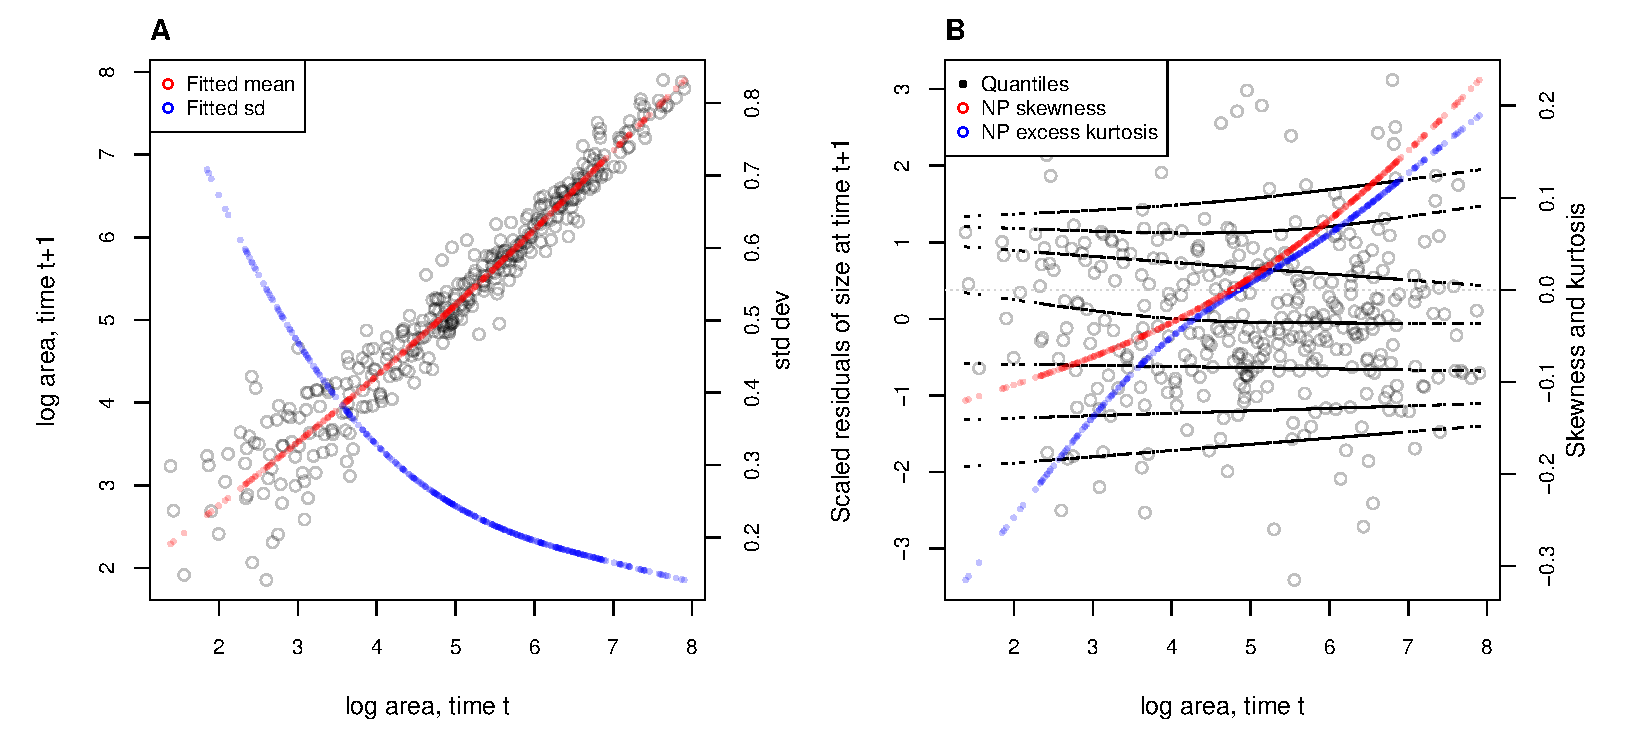
\includegraphics[width=1.0\textwidth]{figures/coral_qgam_diagnostics.pdf}
	\caption{\textbf{A}, Size transition data for sea fan corals, \emph{Gorgonia ventalina}, and fitted gam with mean (red) and standard deviation (blue) of future size conditional on current size.  \textbf{B}, Quantile regressions of scaled residuals on size and nonparametric estimates of skewness (red) and excess kurtosis (blue) derived from them. Black lines in \textbf{B} show the 5th, 10th, 25th, 50th, 75th, 90th, and 95th quantiles. Figure made by script \texttt{AkumalCorals\_qgam.R}.}
	\label{fig:coral_diganostics}
\end{figure} 

There are no blatant signs of trouble in the pilot Gaussian model, but quantile regressions on the scaled residuals, and the NP Skewness and Kurtosis metrics derived from them (Eq. \ref{eqn:NPskew} and \ref{eqn:NPkurt}), suggest deviations from normality (Fig. \ref{fig:coral_diganostics}B).
Specifically, skewness swicthes from negative to positive across the size distribution, with smaller corals more likely to shrink than grow and larger corals more likely to grow than shrink. 
Kurtosis also changes direction over the size distribution, with smaller initial sizes having thinner tails and larger initial sizes having fatter tails than Gaussian. 
Are these apparent deviations from normality 

Consequently, we want to find a better fitting distribution. As noted in the \emph{Introduction} the overall properties of the scaled 
residuals may be misleading if the growth distribution changes as a function of initial size. 
Instead, distribution choice should be guided by properties of distributions conditional on initial size. 
Multiple observations with identical initial sizes will be rare, but we can 
approximate conditional distributions by grouping size transitions with similar initial sizes. 
In fig. \ref{fig:AkumalRollingResiduals}, summary statistics (mean, standard deviation, NP skewness, NP excess kurtosis) 
are plotted (solid points) for a set of overlapping sliding windows, each containing 10\% of the scaled residuals sorted according to initial size. 
The red dashed lines are what we would see if the pilot model were exactly right: zero mean, skewness and excess kurtosis, and 
standard deviation equal to one. Black curves are spline regressions through the points using \texttt{gam}. Panels A) and B) are a ``sanity check'' to verify
that the pilot model was adequate to capture the mean and variance of growth. Panel C) indicates a shift from negative
skew at small sizes to positive skew at larger sizes. Similarly, panel D), reveals that NP kurtosis varies with initial size, 
negative for small fans and positive at large sizes. 

Fitting those properties requires a four-parameter distribution on $(-\infty, \infty)$ that allows nonzero skew and both 
positive and negative excess kurtosis. That narrows the options considerably. 
Of the more than 50 distributions provided in the \textbf{gamlss.dist} package, the options are 
\texttt{EGB2, JSU, GT, SHASH} and four \texttt{SEP} distributions (four different ways of adding skew to the
exponential power distribution). We omit \texttt{SEP2} because it is known to have poorly identified parameters
\citep{diciccio-monti-2004}, which is problematic for choosing the non-Gaussian model structure in the way we propose.   

To choose among the candidate distributions, we sorted the scaled residuals based on initial size into 8 equal-size bins, 
and used maximum likelihood to fit all candidate distributions to each bin.\footnote{Our function \texttt{gamlssMaxlik} 
in online script \texttt{fitChosenDists.R} is
patterned after the \texttt{gamlss} function \texttt{gamlssML}, but uses the \texttt{maxLik} function from the \textbf{maxLik}
package \citep{maxLik-package}, and repeated optimization from different starting values, to increase the reliability of the results.} 
As all distributions have the same number of parameters, comparison of maximized likelihoods is equivalent to comparing AIC values. 
With the exception of \texttt{EGB2} all distributions had very similar maximized likelihoods for all bins; the best overall (summed
likelihood) was \texttt{SEP1}, so we proceeded with \texttt{SEP1}. With 5 bins instead of 8 the outcome was the same. 

Most four-parameter distributions have the inconvenient property that their parameters are \emph{not} the mean, standard deviation, skew,
and kurtosis of the distribution. This happens because (for example) introducing nonzero skew changes the mean and the kurtosis. 
So to see how distribution parameters vary as a function of initial size, instead of inspecting fig. \ref{fig:AkumalRollingResiduals}, we need
to look directly at how parameters vary as a function of initial size. As before, we did this by binning the data based on initial sizee, 
and fitting an \texttt{SEP1} distribution to the subsequent size values in each data subset. Note, 
in fig. \ref{fig:AkumalRollingResiduals} we used scaled residuals as the response variable, 
to minimize how variation in mean and standard deviation within a bin would affect the skew and kurtosis. 
Now, because all four distribution parameters interact to determine the distribution, we need to fit all 
four simultaneously to the data in each bin. 

\begin{figure}[tbp]
\centering
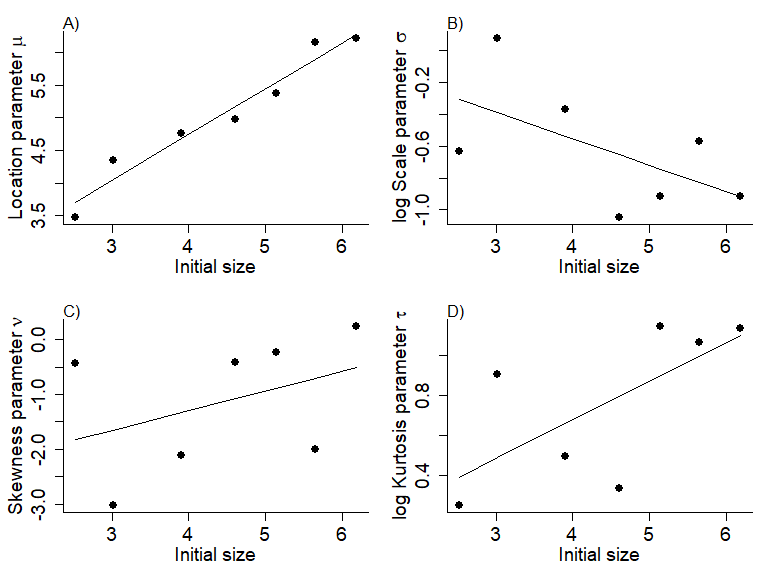
\includegraphics[width=0.8\textwidth]{figures/AkumalRollingSEP1pars.png}
\caption{Binned data SEP1 parameter estimates for growth distributions of sea fan corals, \emph{Gorgonia ventalina}. 
Figure made by scripts \texttt{AkumalCorals.R} and \texttt{Diagnostics.R}.}
\label{fig:AkumalRollingSEP1pars}
\end{figure} 

As expected from the pilot Gaussian fit, the location parameter $\mu$, the log of the scale parameters $\sigma$, the 
skewness parameter $\nu$ and log of the kurtosis parameter $\tau$ all appear to vary linearly with initial size 
(log is the default link function for $\sigma$ and $\tau$ in \texttt{SEP1} because both must be positive).
The corresponding overall growth model is an \texttt{SEP1} distribution in 
which $\mu, \log \sigma, \nu$ and $\log \tau$ are all linear functions of initial size.
However, following our suggested workflow, we specify $\mu$ as a quadratic function of initial size because that relationship
was found to be nonlinear in the pilot Gaussian model. This model is easily fitted by maximum likelihood, 
using the pilot Gaussian fit and the values plotted in fig. \ref{fig:AkumalRollingSEP1pars} to 
inform the starting parameter values. The quadratic term for $\mu$ proved to be highly significant
($p<0.001$ based on the asymptotic standard error from the inverse Hessian). 

\begin{figure}[tbp]
\centering
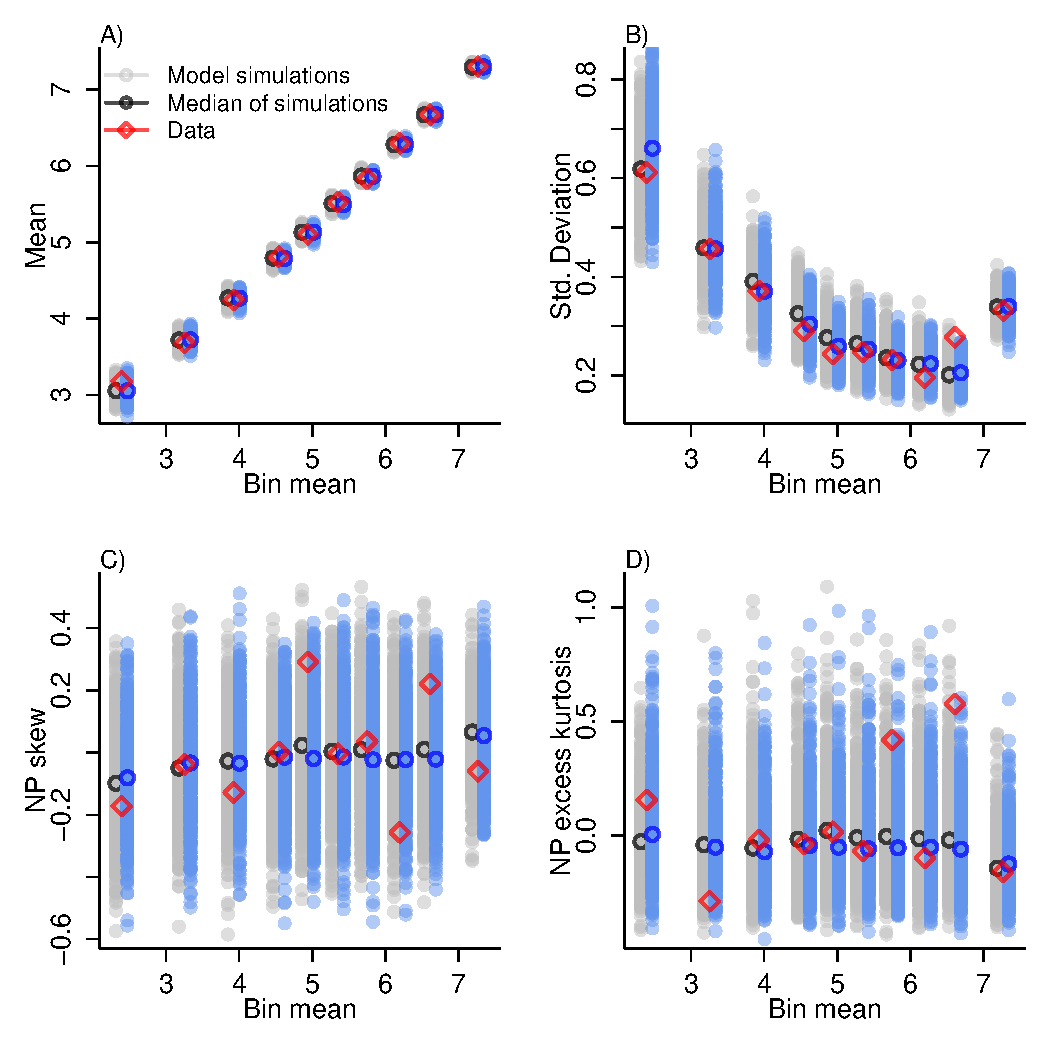
\includegraphics[width=.95\textwidth]{figures/CoralMomentsComparePlot.pdf}
\caption{Binned data comparison of moments between 500 simulations of the fitted SEP1 model (grey, black circles), 500 simulations
of the fitted Gaussian model (light blue and blue circles), and the actual data (red diamonds) for sea fan corals \emph{G. ventalina}. 
Grey and light blue circles show the moments for each of 500 replicate simulations,
in which the fitted growth models were applied to all initial sizes in the empirical data sets, and black/dark blue circles are the mean
across replicates. Red diamonds are values for the data. Bins are defined by initial size. Figure
made by scripts \texttt{Akumal Corals.R} and \texttt{Diagnostics.R}.}
\label{fig:CoralMomentsCompare}
\end{figure} 

The ``acid test'' of a growth model is that simulations from the fitted model should look like the real data. 
To implement that criterion, we compared simulated and actual data with respect to moments of the distribution
of subsequent size, again using a series of bins defined by initial size to account for how those quantiles vary
with initial size. As a benchmark, we did the same for simulations of the pilot Gaussian model. The results, in  
fig. \ref{fig:CoralMomentsCompare}, \new{show depressingly small differences between the Gaussian and non-Gaussian models.} 
 
What, then, have we gained by fitting a better growth model? Fig. \ref{CoralKernelCompare}A
compares the predicted distributions of subsequent size in the fitted model and Gaussian pilot models, for the median size of a new recruit 
(leftmost pair of curves), the median initial size (central curves), and the 95th percentile of initial size in the data (rightmost
curves). Differences are most pronounced for recruits, which have better odds of growing (leading to earlier reproduction and higher
survival) in the fitted model, small at intermediate sizes where the skew and excess kurtosis are both small (fig. \ref{fig:AkumalRollingResiduals}CD),
and larger again at high sizes where the fitted model is leptokurtic. Fig. \ref{fig:CoralKernelCompare}B shows the predicted steady-state size
distributions resulting from a constant unit input of recruits. The main difference is that the pilot model projects fewer individuals at
or near the modal size; overall, the fitted model predicts 7\% more individuals at steady-state. Equivalently, the fitted
model predicts a 7\% higher mean lifespan, 19.0 years vs. 17.7 in the pilot Gaussian model. 

\begin{figure}[tbp]
\centering
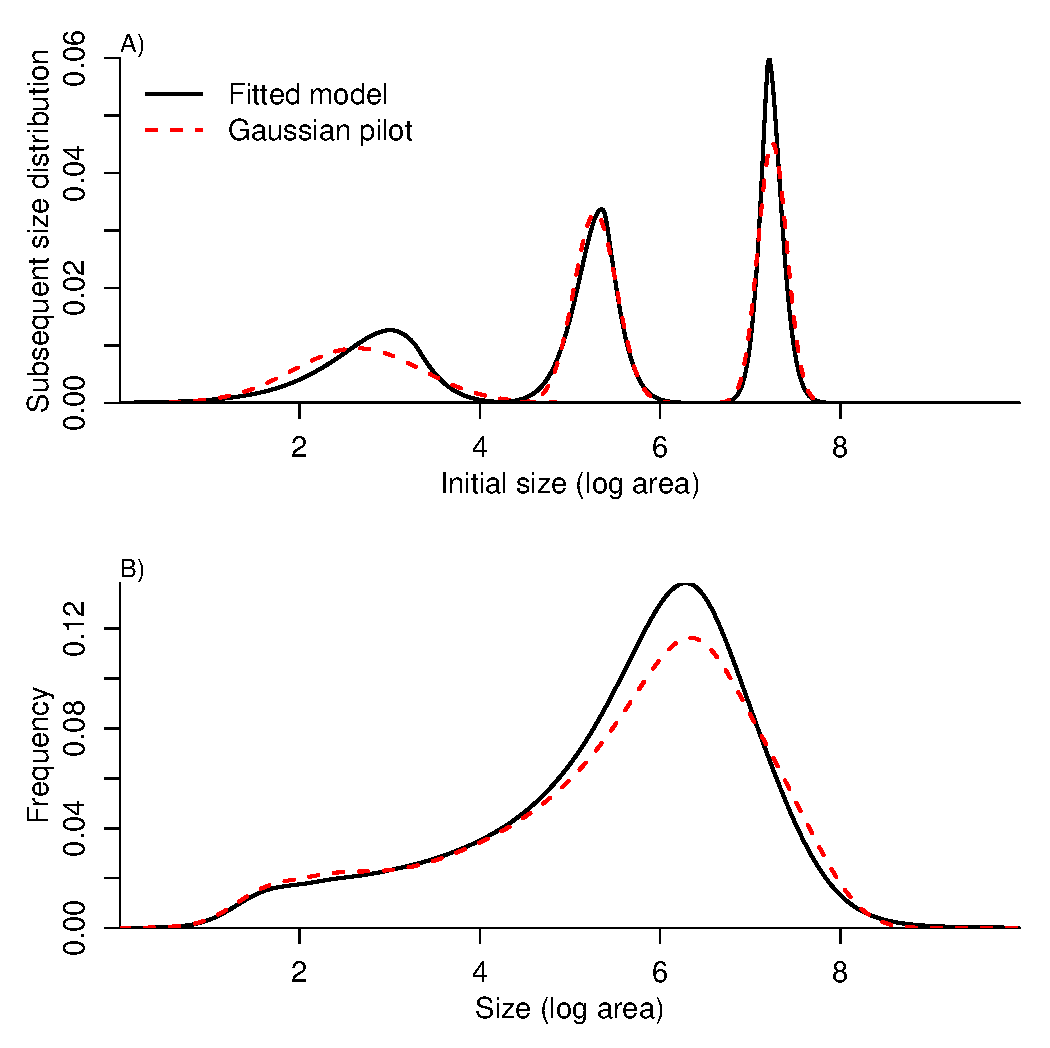
\includegraphics[width=.9\textwidth]{figures/CoralKernelCompare.pdf}
\caption{Comparisons between the fitted \texttt{SEP1} growth model (solid black curves) and the Gaussian pilot model (dashed red curves)
for sea fans \emph{G. ventalina}. A) Predicted frequency distributions of size in year $t+1$ for three different values of size in 
year $t$. The leftmost pair of curves are for initial size equal to the median size of a new recruit (data from \citep{bruno-etal-2011}); 
central pair is for the median initial size of uninfected individuals; rightmost pair are for the 95th percentile initial size for uninfected
individuals. B) Steady-state size distributions resulting from a constant unit input of new recruits. As in \citet{bruno-etal-2011} we
assume that larvae are very widely dispersed, so that the number of recruits arriving at any one location is independent of the local population
abundance or structure. Size distribution of recruits was described by a kernel density estimate based on the (sadly, only $n=9$) measured sizes
of known new recruits. Figure made by script \texttt{AkumalCoralsIPMs.R}.}
\label{fig:CoralKernelCompare}
\end{figure}  

\new{We used \texttt{gam} to fit the pilot Gaussian model because that obviated model selection on the mean and variance functions.
However, \texttt{gam} should be used with caution. Nonparametric regression models notoriously ``wag their tails'' because the ends of 
the fitted curve can be pulled close to the outermost data points. This is especially problematic for growth modeling, because data are typically 
sparse near the top and bottom of the size range. To minimize the risk of overfitting we have used \texttt{gamma=1.4} to overweight
model degrees of freedom, as suggested by \citet[][sec. 3.2]{gu-2013}. But it is always important to 
plot the fitted splines and make sure they do not wag unrealistically. If they do, the pilot model 
can be fitted with parametric regression, as we illustrate in our cactus and creosote bush case studies.}

\clearpage   

\section{Case study: cactus, \emph{Cylindriopuntia imbricata}}
The next case study, focusing on the tree cholla cactus \emph{Cylindriopuntia imbricata} at the Sevilleta Long-Term Ecological Research site in central New Mexico, adds an important new feature on top of the simple size-dependent regressions in the previous study: random effects associated with temporal (year) and spatial (plot) environmental heterogeneity. 
This long-term study of cactus demography was initiated in 2004 and different subsets of the data have been analyzed in various IPM studies, all using Gaussian growth kernels  \citep{miller2009impacts,czachurademographic,compagnoni2016effect,ohm2014balancing,elderd2016quantifying}.
In fact, \citep{elderd2016quantifying} presented a Gaussian growth model fit to the cactus data as an example of a well fit growth function, based on a marginal distribution of residuals that appeared approximately Gaussian and posterior predictive checks (PPCs) of a Bayesian model that suggested consistency between the real data and data simulated from the fitted model (Fig. 4 in \citep{elderd2016quantifying}). 
While PPCs and the associated ``Bayesian P-value'' are popular diagnostic tools, they are often considered to be too conservative \citep{conn2018guide,zhang2014comparative}, failing to reject marginally bad models even though they are very effective in rejecting models that are terrible.
The choice of discrepancy function (the statistic used to describe real and simulated data) can also be limiting: in our previous work, we used a discrepancy function focused on variance (the sum of the squared residuals), so we had a built-in blind-spot for mismatches in higher moments.
In the clarity of hindsight, the PPC gave a false sense of security; the Gaussian was a poor choice all along.

The data for this new analysis include $5203$ size transition observations from $924$ unique individuals spanning nine transition years (2009--2017) and eight $30m$-by-$30m$ plots (we excluded earlier years of data corresponding to a different cohort of plants from a different set of locations). 
Following previous studies, we quantified size as the natural logarithm of plant volume ($cm^3$), derived from height and width measurements. 

\subsection{A pilot Gaussian model}
We begin the growth modeling workflow with a simple mixed model for size in year $t+1$ as a function of size in year $t$, with random intercepts for year and plot and assuming normally distributed residuals. 
We considered four candidate models, with and without a quadratic term in the predictor for the mean and with residual variance as a function of either initial size or the model's fitted value (which includes initial size plus the random effects).
We allowed for non-constant variance by iterively re-fitting the models with weights based on a second-order polynomial that related the $SD$ of the residuals to initial size or fitted values. 
We iterated until there was effectively no change in the model weights, indicating convergence on maximum likelihood parameter estimates for the coefficients of the mean and $SD$ linear predictors. 

The best-fit model from this pilot analysis included the quadratic term for the mean and residual variance as a function of initial size. 
However, while the standardized residuals from this model are approximatley mean zero and unit variance (as they should be), there are clear deviations from normality in the higher moments: negative skew (decreases in size were more common than increases, visible in the raw data [Fig. \ref{fig:cactus_kernel_gaussian}]) and positive excess kurtosis, both greater at smaller sizes and minimal at larger sizes (Fig. \ref{fig:cactus_rolling_moments}). 

\begin{figure}
\centering
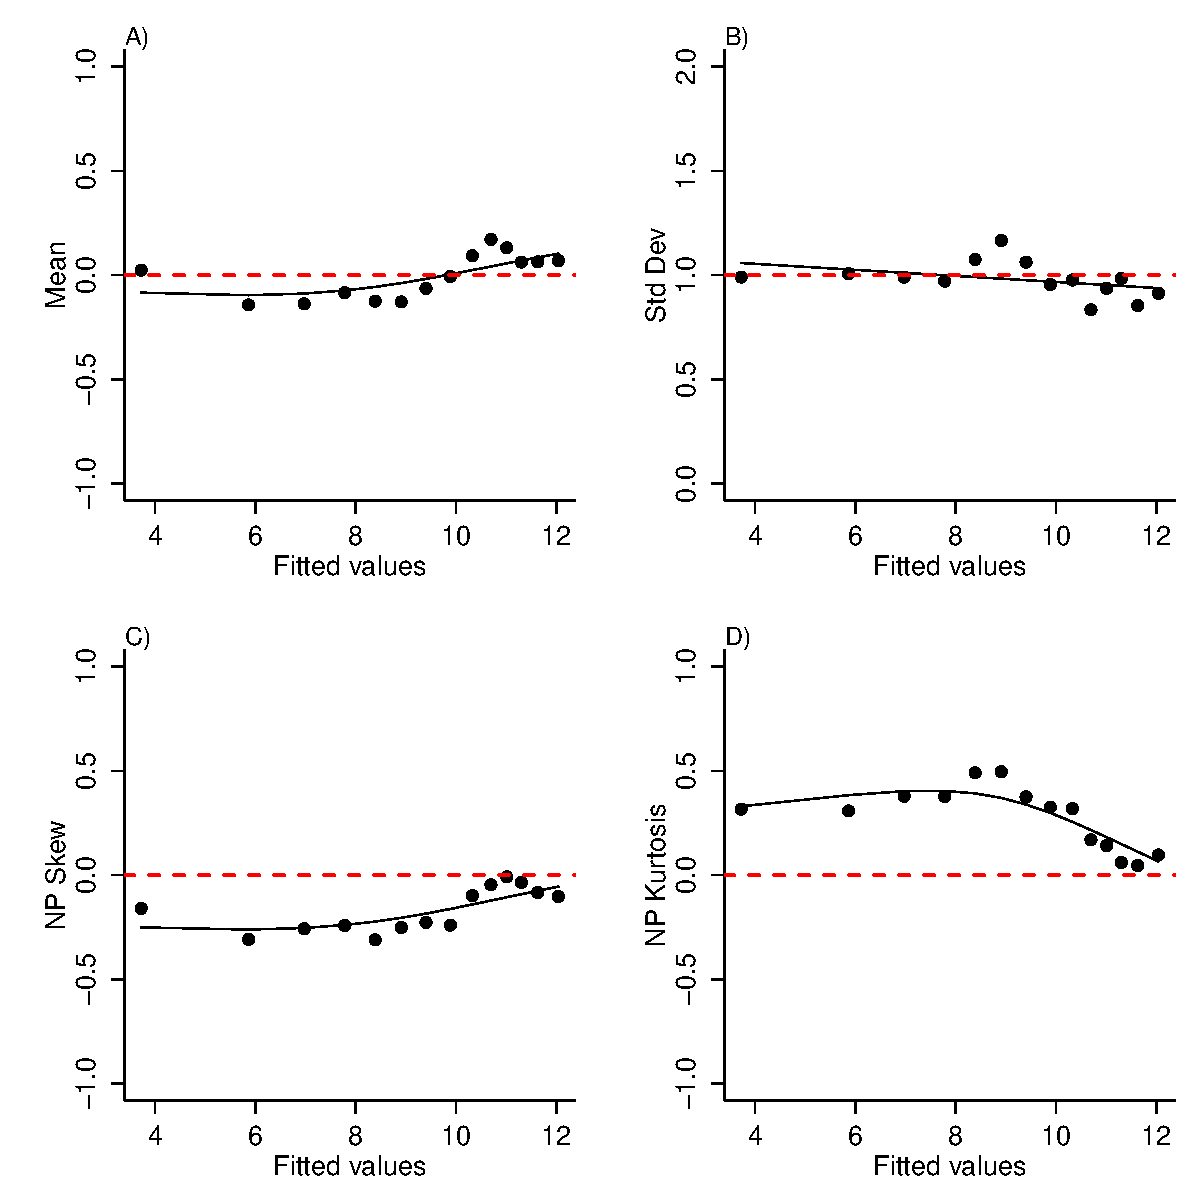
\includegraphics[width=0.75\textwidth]{figures/cactus_rolling_moments}
\caption{Rolling-moment analysis of standardized residual from a Gaussian fit to the cactus growth data. Red dashed lines indicate the Gaussian expectation. These data show skewness and kurtosis that deviate from Gaussian.}
\label{fig:cactus_rolling_moments}
\end{figure} 

\subsection{An improved growth model}
To better capture size transitions, we need a distribution with negative skew and positive excess kurtosis, but both of which may be negligible at some sizes. 
Appropriate candidates include Johnson's $S_{U}$ distribution, which is limited to positive excess kurtosis, and the sinh-arcsinh (SHASH) and skewed power exponential distributions, which can vary from leptokurtic to platykurtic (Fig. \ref{fig:workflow}). 
As above, we divided the standardized residuals into discrete bins of initial size and fit competing distributions to each data subset using our function \texttt{gamlssMaxlik()}.
We found that Johnson's $S_{U}$ distribution (\texttt{JSU} in \textbf{gamlss}) was favored over most of the size distribution, particularly the larger sizes. 
However, at smaller sizes, the SHASH distribution was favored. 
They are both four-parameter distributions but the SHASH is more flexible than the JSU, capable of capturing a greater range of possible kurtosis for a given amount of skew\tom{}{This comes from Steve's NPSkewKurtosisRanges.pdf}. 
We ultimately settled on the SHASH distribution, but only after first trying the JSU and proceeding through the workflow (Fig. \ref{fig:workflow}). 
We were unsatisfied with the correspondence between real and simulated data in the final step, so we followed the re-iteration loop back to "choose a better distribution", this time the SHASH. 
To keep this section concise, we do not fully narrate that re-iteration loop, but we expect it will be a common feature of many growth analyses. 

To guide the final fit, we visualized parameter estimates of the SHASH distribution across bins of initial size, which suggested second-order polynomials for the parameters that control variance, skew, and kurtosis (Fig. \ref{fig:cactus_binned_SHASH}). 
The final likelihood model was thus:
\begin{figure}
\centering
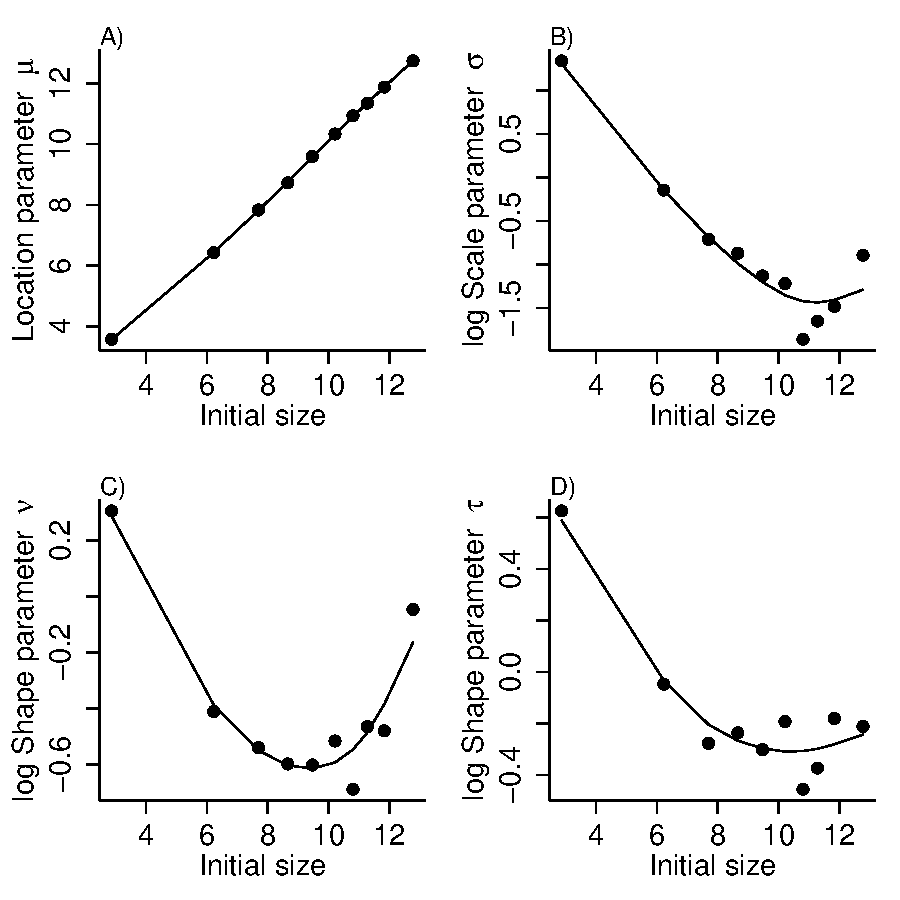
\includegraphics[width=0.75\textwidth]{figures/cactus_binned_SHASH}
\caption{Parameter estimates of the \texttt{SHASH} distributions fit to cactus growth data in discrete bins of initial size.}
\label{fig:cactus_binned_SHASH}
\end{figure} 

\begin{lstlisting}
LogLik=function(pars,response,U){
  pars1 = pars[1:ncol(U)]; pars2=pars[-(1:ncol(U))];
  mu = U%*%pars1;  
  val = dJSU(x = response, 
             mu=mu,
             sigma = exp(pars2[1] + pars2[2]*x + pars2[3]*x^2), 
             nu = pars2[4] + pars2[5]*x  + pars2[3]*x^2, 
             tau = exp(pars2[6] + pars2[7]*x + pars2[8]*x^2), log=T) 
  return(val)
} 
\end{lstlisting}
Here, \texttt{response} is future size and \texttt{U} is the model matrix for the location parameter of the SHASH, derived from the mean of the best-fit Gaussian model, but now converting random effects of years and plots to fixed effects:
\begin{lstlisting}
U=model.matrix(~  0 + year_t + plot + log(vol_t)+ I(log(vol_t)^2), data=CYIM)
\end{lstlisting}

We can use the `shrinkage' methods described in Appendix S.1 to estimate the variance terms associated with year and plot effects, even though they are fit here as fixed effects.
There is a tedious but not insurmountable complication that can arise in models with multiple random effects, as in this one.
By supressing the intercept in the model matrix (the zero after the tilde), we get parameter estimates for each year rather than offsets relative to a baseline year.
However, because there is the additional effect of plot, all of the year effects are conditioned on the first level of the plot factor variable (plot 1) and the remaining plot coefficients are offsets of plot 1.
The parameter estimate for plot 1 is therefore the mean of the year estimates, but there is no way to calculate its standard error. 
We estimate the plot variance \tom{excluding plot 1}{A very unsatisfying feature of this analysis. I've tried flipping the order so that plots are conditioned on year 1, but when I do it this way \texttt{sigma2.hat} for plot is negative. Not totally unreasonable because the plot effects are small relative to year effects, but still annoying. Steve has mentioned that we might get around this by abandoning the model.matrix function but I don't see how. We cannot get unconditional estimates of plot and year effects without adding a parameter to the model, and that parameter is unidentifiable.}, a possible source of bias the variance estimate. 
The random effects estimated via the shrinkage method correspond well with those from the original Gaussian mixed model, particularly for year effects (Fig. \ref{fig:cactus_rfx_compare}A). 
Plot effects were less tightly correlated but there was also less variance across plots than there was across years (Fig. \ref{fig:cactus_rfx_compare}B). 

\begin{figure}
\centering
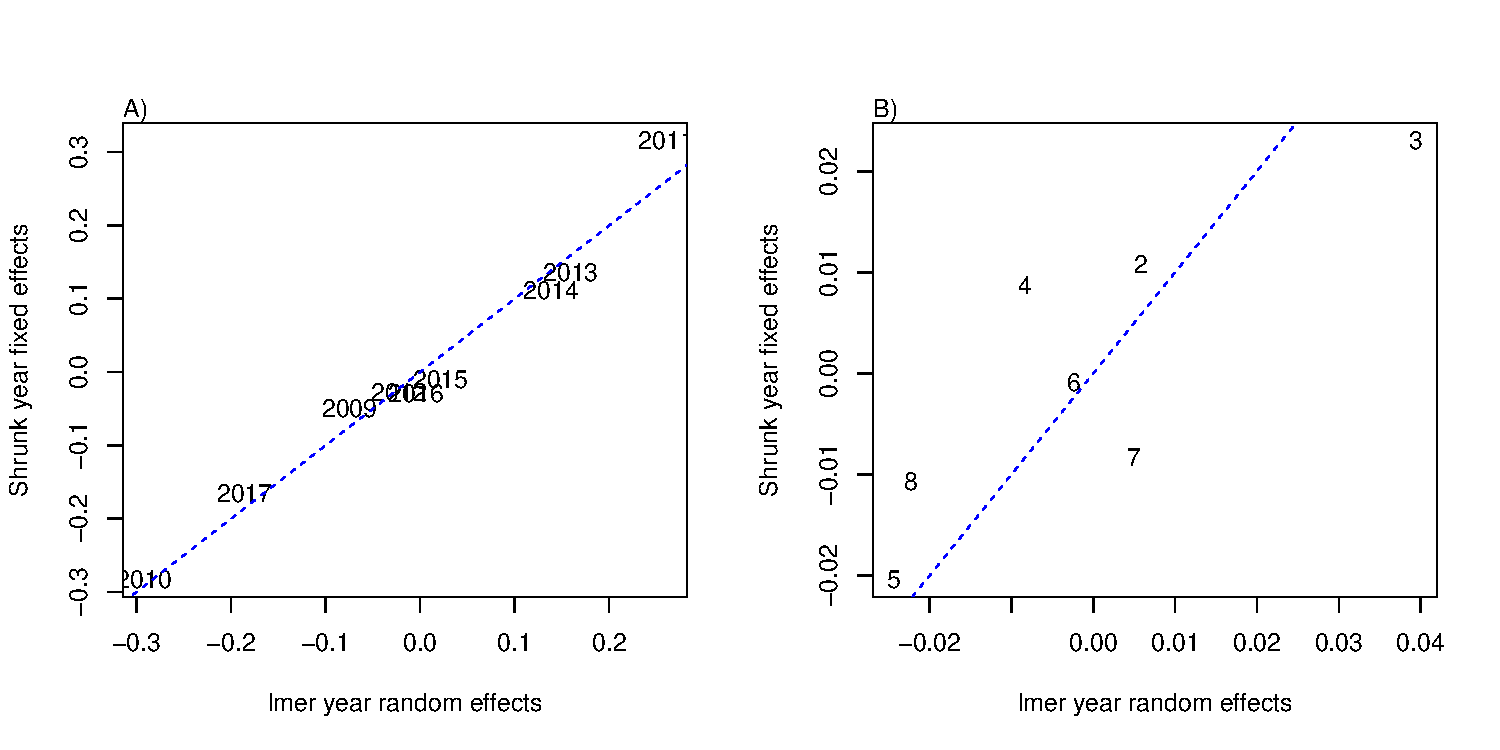
\includegraphics[width=\textwidth]{figures/cactus_rfx_compare}
\caption{Comparison of year (A) and plot (B) random effects from `shrinking' fixed-effect estimates (y-axes) vs. \textbf{lme4} mixed models (x-axes) for cactus data set.}
\label{fig:cactus_rfx_compare}
\end{figure} 

Simulations of the final SHASH model -- the final step of the workflow -- indicate that it describes the cactus growth data well (Fig. \ref{fig:cactus_sim_moments}). 
The SHASH model did not provide a noticeable improvement over the Gaussian model in terms of mean and variance of size transitions (Fig. \ref{fig:cactus_sim_moments}A,B).
This is expected, since an appropriately specified Gaussian model with non-constant variance should be able to accommodate this type of complexity.
It is in skewness and kurtosis that the SHASH really shines (Fig. \ref{fig:cactus_sim_moments}C,D), effectively capturing observed trends in these features of size transitions. 

\begin{figure}
\centering
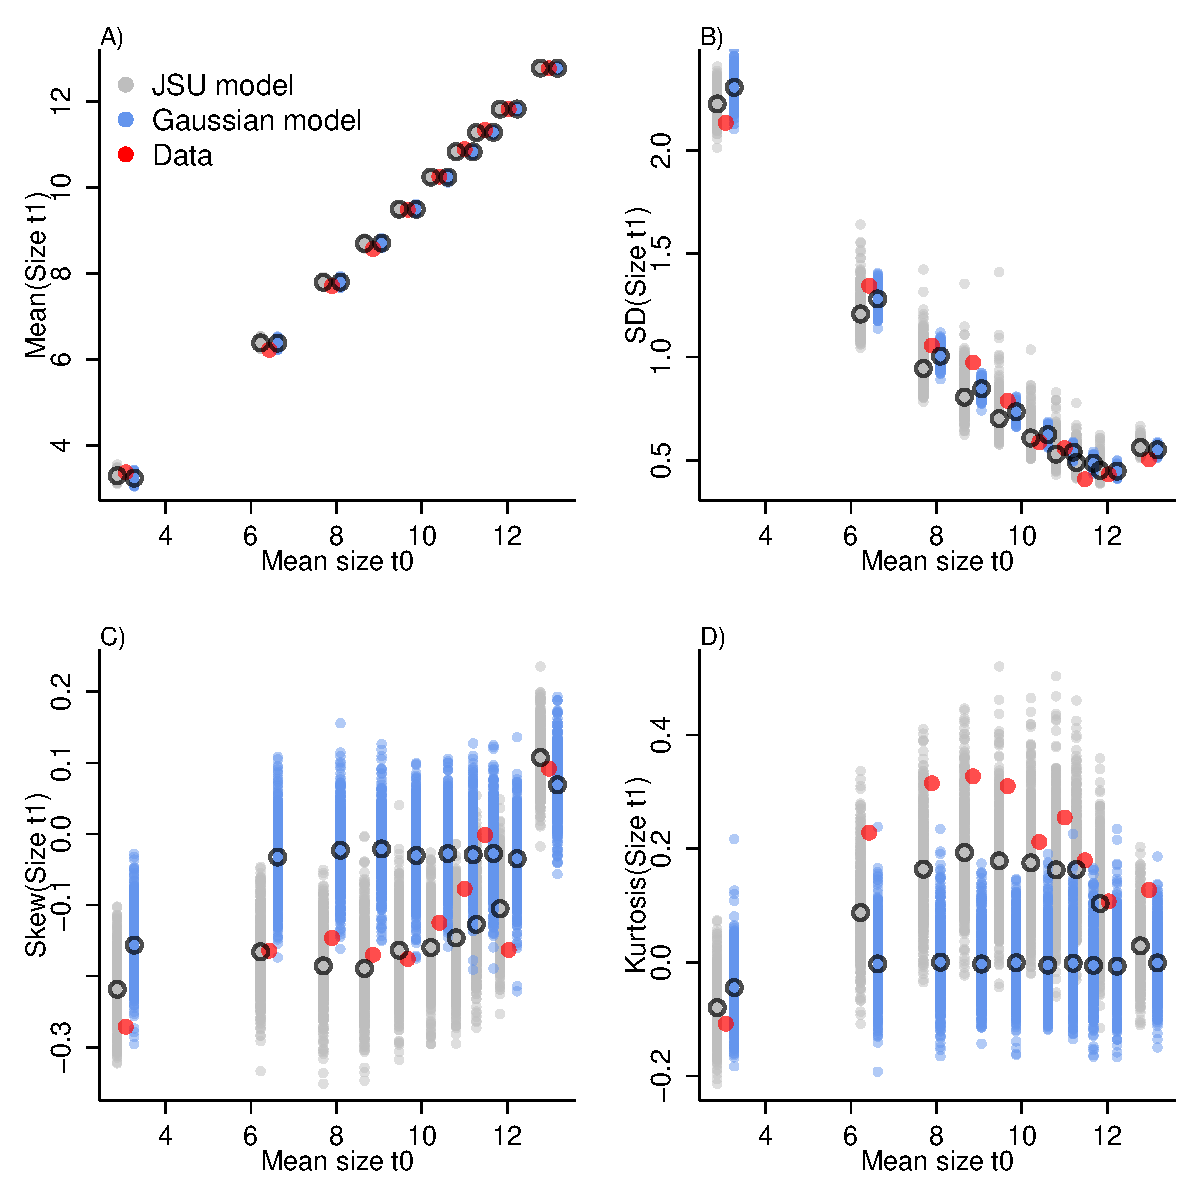
\includegraphics[width=\textwidth]{figures/cactus_sim_moments}
\caption{Simulated data from SHASH and Gaussian growth kernels compared to cactus growth data to which the models were fit.}
\label{fig:cactus_sim_moments}
\end{figure} 

\subsection{Consequences of improved growth modeling for IPM predictions}
Finally, we can ask how the improvements we have made to modeling cactus growth affect inferences from the full IPM.
Details of IPM construction and analysis are provided in Appendix \tom{\#}{Need to do. Maybe we can have one appendix for all the IPMs.}.
Our previous IPM analyses of this system have consistently shown asymptotic population growth rates below replacement-level ($\lambda < 1$).
Our new results with the improved SHASH growth kernel are qualitatively consistent with these results.
However the SHASH growth kernel predicts a much faster rate of decline -- a $9\%$ difference in annual change -- than the Gaussian, holding all else equal ($\lambda_{SHASH} = 0.901$ vs. $\lambda_{Gaussian} = 0.995$).
The SHASH also predicts a very different and much smaller stable size distribution (SSD) than does the Gaussian (Fig. \ref{fig:cactus_ssd}). 
The observed size distribution falls in between the two predictions, suggesting that, either way, this population is not at its stable distribution. 
The difference in predictions of the two IPMs is driven by contrasting size transitions of large plants (Fig. \ref{fig:cactus_growth_compare}).
This contrast is driven by skew and kurtosis, since the mean and variance of the SHASH and Gaussian models were nearly identical for large sizes (Fig. \ref{fig:cactus_sim_moments}). 
The Gaussian growth kernel over-predicts size transitions at large sizes, and this leads to the larger median size at SSD and also the smaller peak corresponding to new recruits, since reproductive output is strongly size-dependent. 
This peak disappears from the SHASH SSD because reproductive output is strongly size dependent, and the SHASH growth kernel predicts that transitions to the largest sizes are less likely. 
\begin{figure}
\centering
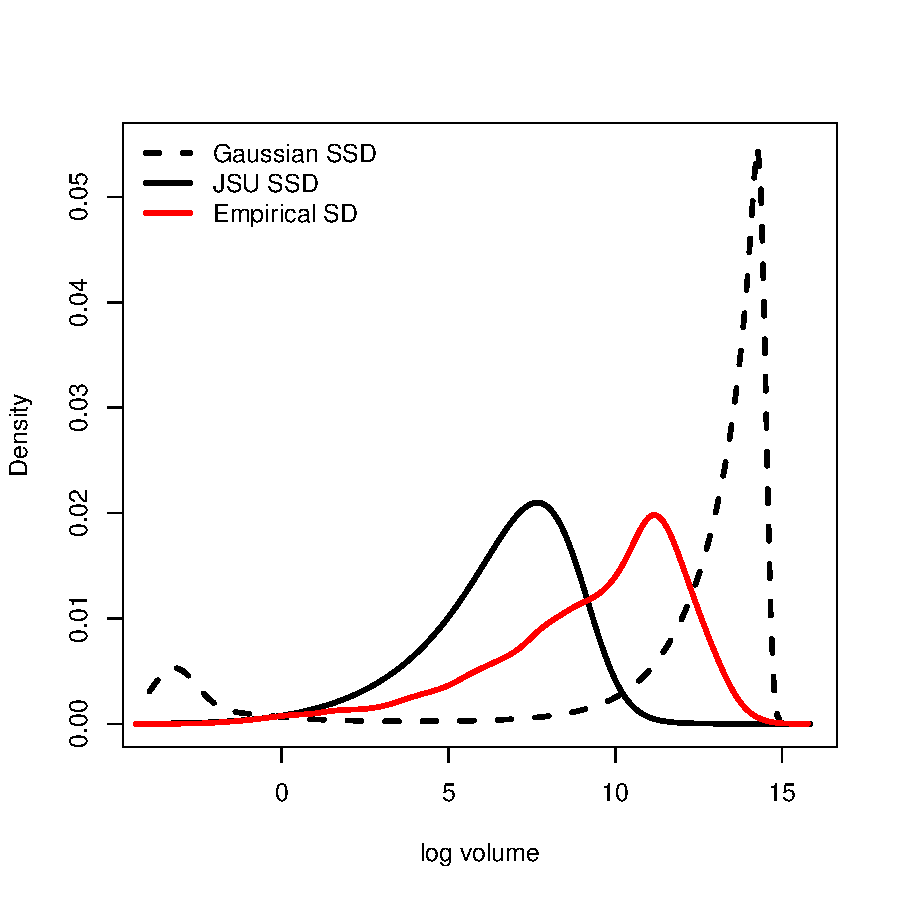
\includegraphics[width=0.75\textwidth]{figures/cactus_ssd}
\caption{Predicted and observed size distributions of tree cholla cactus.}
\label{fig:cactus_ssd}
\end{figure} 
 
 \begin{figure}
\centering
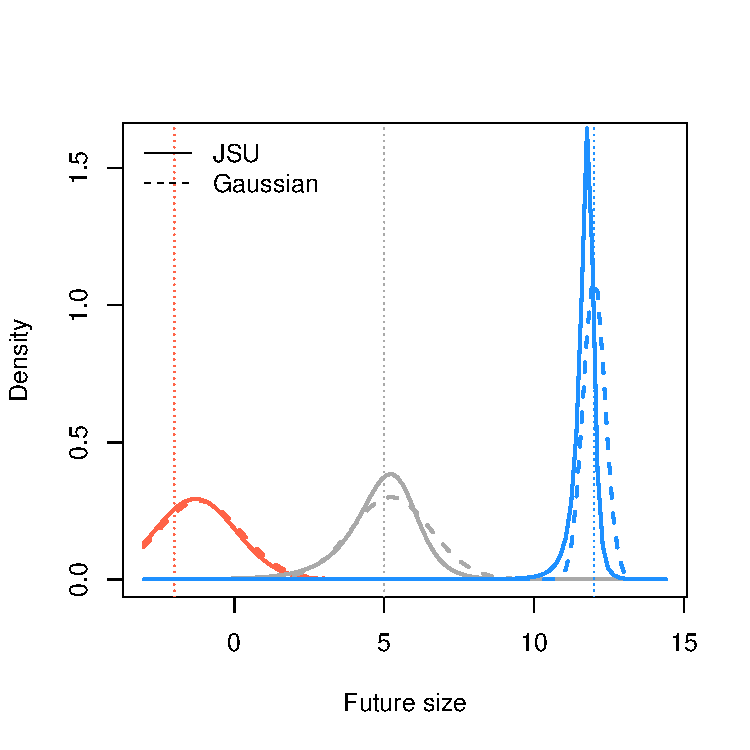
\includegraphics[width=0.75\textwidth]{figures/cactus_growth_compare}
\caption{Predicted probability of future size given three initial sizes indicated by vertical lines.}
\label{fig:cactus_growth_compare}
\end{figure} 

\clearpage   

\section{Case study: bunchgrass, \emph{Pseudoroegneria spicata}}

We again consider a species where one of us is the offender -- initially using the default model because 
it was hard to do better at the time \citep{adler-etal-2010}, but sticking with it 
\citep[e.g.,][]{Tredennick2018, Adler-2018} when it would have been easy to do better. 

We used the most recently curated version of the data \citep[][at doi.org/10.5061/dryad.96dn293]{Adler-2018},
both legacy (22 annual transitions between 1926 and 1957) and modern (8 annual transitions from
2008 to 2016, excluding moisture manipulation treatments). We excluded seedlings, which require separate models
\citep{Chu-2014a, Chu-2015, snyder-ellner-2018}, and individuals mapped as ``too small to measure'' that should be modeled separately
as a discrete size category (though in the past we have not done that). The measure of plant size was log basal cover. 

Based on past analyses, (1) we did not distinguish between historical and 
modern Control treatments \citep{Adler-2018} (2) we included size by year interactions with year-specific slope and intercept
for a linear relationship between current and future size (log basal cover); (3) Quadrat group (labeling sets of spatially
nearby quadrats), Treatment (Control or Shrub removal) and competition with other species were included as covariates. 
As in past models, competition was measured by distance-weighted cover of competing species, using nonparametric competition
kernels estimated from the data \citep{Teller-2016}. 

Results: \begin{enumerate}

\item The Gaussian pilot model was fitted using \texttt{gam}, with spline terms for the effect of initial size on the
mean subsequent size, and for the standard deviation. Based on past analyses, (1) the measure of size was log basal cover; 
(2) We did not distinguish between historical and contemporary Control treatments \citep{Adler-2018}; (3) the model 
included size by year interactions, with year-specific slope and intercept for a linear effect of current size on
future size; (3) quadrat group (labeling sets of spatially nearby quadrats), Treatment (Control or Shrub Removal) and 
competition with other species were included as covariates. As in past models, competition was measured by distance-weighted 
cover of competing species, using nonparametric competition kernels estimated from the data \citep{Teller-2016}. 

\item Model selection for the pilot Gaussian model was thus limited to (1) reducing the number of competition
terms by combining or dropping species, and (2) choosing between two options for the variance: dependence on 
initial size, or on the predicted mean subsequent size. The latter option is not directly available in \texttt{gam}, but was done
through iterative re-fitting Model selection was based on AIC values reported by \texttt{gam}). Growth variance depending on
the linear predictor was strongly favored ($\Delta$ AIC $\approx 50$). The selected competition model had  
three competition covariates: (1) cover of the shrub \emph{Artemisia tripartita}, (2) cover of the other two dominant 
bunchgrasses combined, and (3) cover of all other species combined. 

\item The set of all scaled residuals was non-Gaussian, based on quantile-quantile plot, mostly in the lower tail. Statistical tests
confirmed that the standardized residuals are non-Gaussian (all $P<0.001$). 

\item Rolling moments diagnostics on the scaled residuals (Fig. \ref{fig:rollingMomentsPSSP}) confirm that the mean 
and SD are nearly constant as a function of the fitted value, as they should be. The small trend in the mean shows that the 
regression coefficients are slightly biased, which is not unexpected because the Gaussian assumption is violated. 
The trends in skew and kurtosis are too big to ignore.  

\begin{figure}[tbp]
\centering
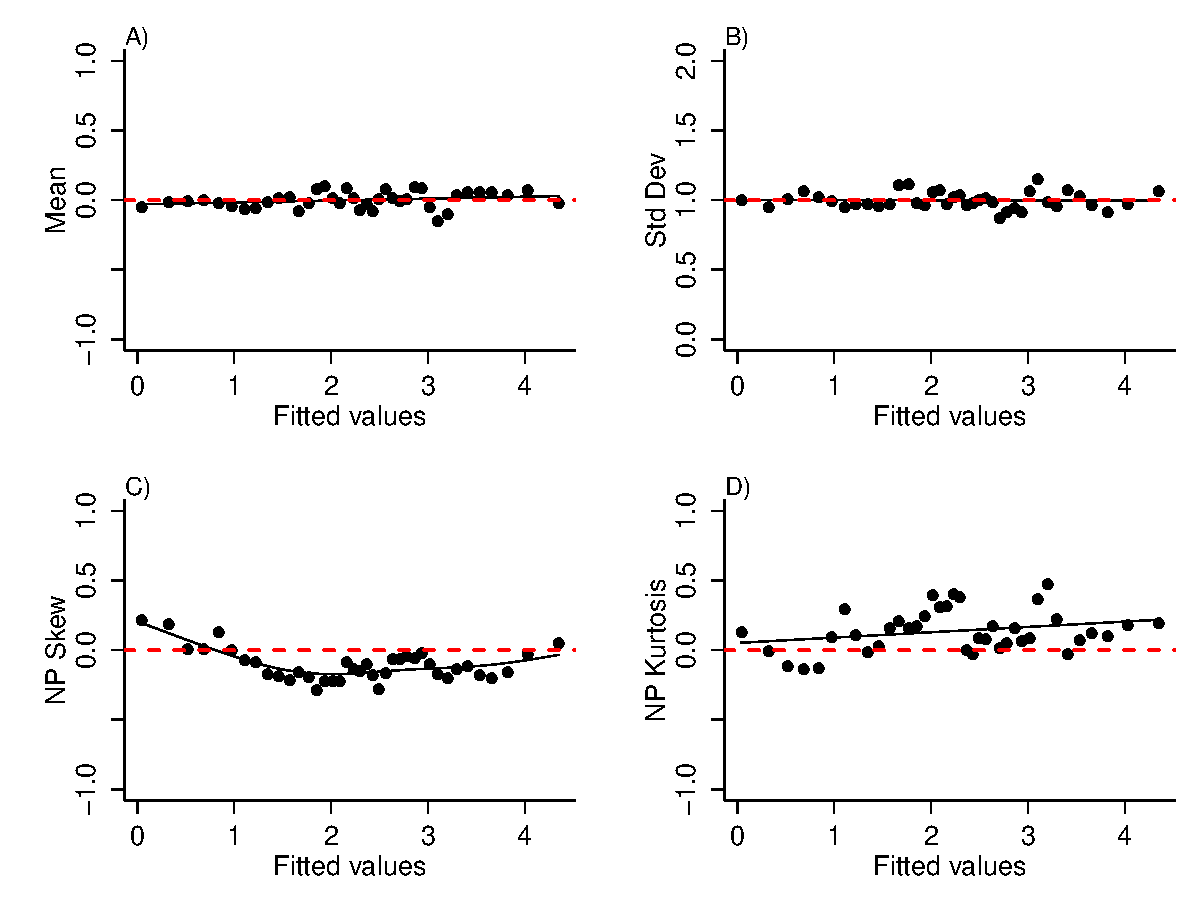
\includegraphics[width=.9\textwidth]{figures/RollingNPMomentsPSSP.pdf}
\caption{Rolling moments of scaled residuals from the pilot model, as a function of fitted
values, for \emph{P. spicata}. The dashed red lines are the value expected if the pilot model fits the
data.}
\label{fig:rollingMomentsPSSP}
\end{figure} 

\item What distribution families can accomodate the features in Fig. \ref{fig:rollingMomentsPSSP}?
We need at least 4 parameters (to allow skew and excess kurtosis), and both postive and zero excess kurtosis must be 
possible. In JSU and skew $t$ and that makes fitting problematic, because zero excess kurtosis only occurs as a limit, not at 
any actually possible parameter values ($df \to \infty$ for $t$, and $\tau \to 0$ for JSU). Comparison was therefore limited
to \texttt{SHASH,SHASHo,SEP1,SEP3,SEP4} -- not \texttt{SEP2} for the reasons noted above. The winner was SHASH. 

\begin{figure}[tbp]
\centering
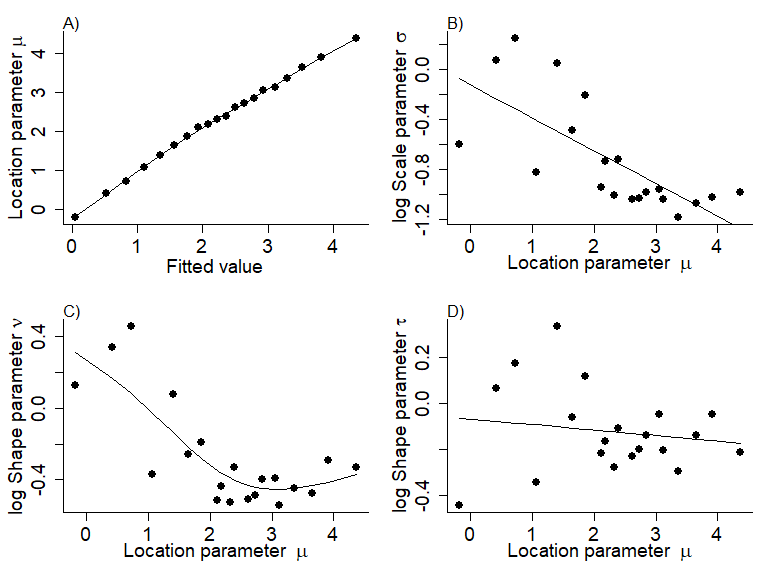
\includegraphics[width=.9\textwidth]{figures/RollingSHASHparsPSSP.png}
\caption{Binned data SHASH parameters plot for \emph{P. spicata}. }
\label{fig:rollingSHASHparsPSSP}
\end{figure} 

\item Now we need to model the size-dependence of the SHASH distribution parameters. In the pilot model, $\sigma$ as a function
of fitted value was strongly favored or $\sigma$ as a function of initial size. We retain that structure in the SHASH model. 
The data were therefore binned based on fitted values of the pilot model, and a SHASH distribution was fitted to each bin. 
fig. \ref{fig:rollingSHASHparsPSSP}. Panel A), $\mu$ as a function of the fitted values, doesn't really inform the 
modeling, but it shows that it is safe to regard $\mu$ as equivalent to the ``fitted value'' in the pilot model. 
The other plots tell us how the other distribution parameters should be modeled as a function of $\mu$. $\log \tau$ is quadratic,
and $log \nu$ is linear. 
 

\begin{figure}[tbp]
\centering
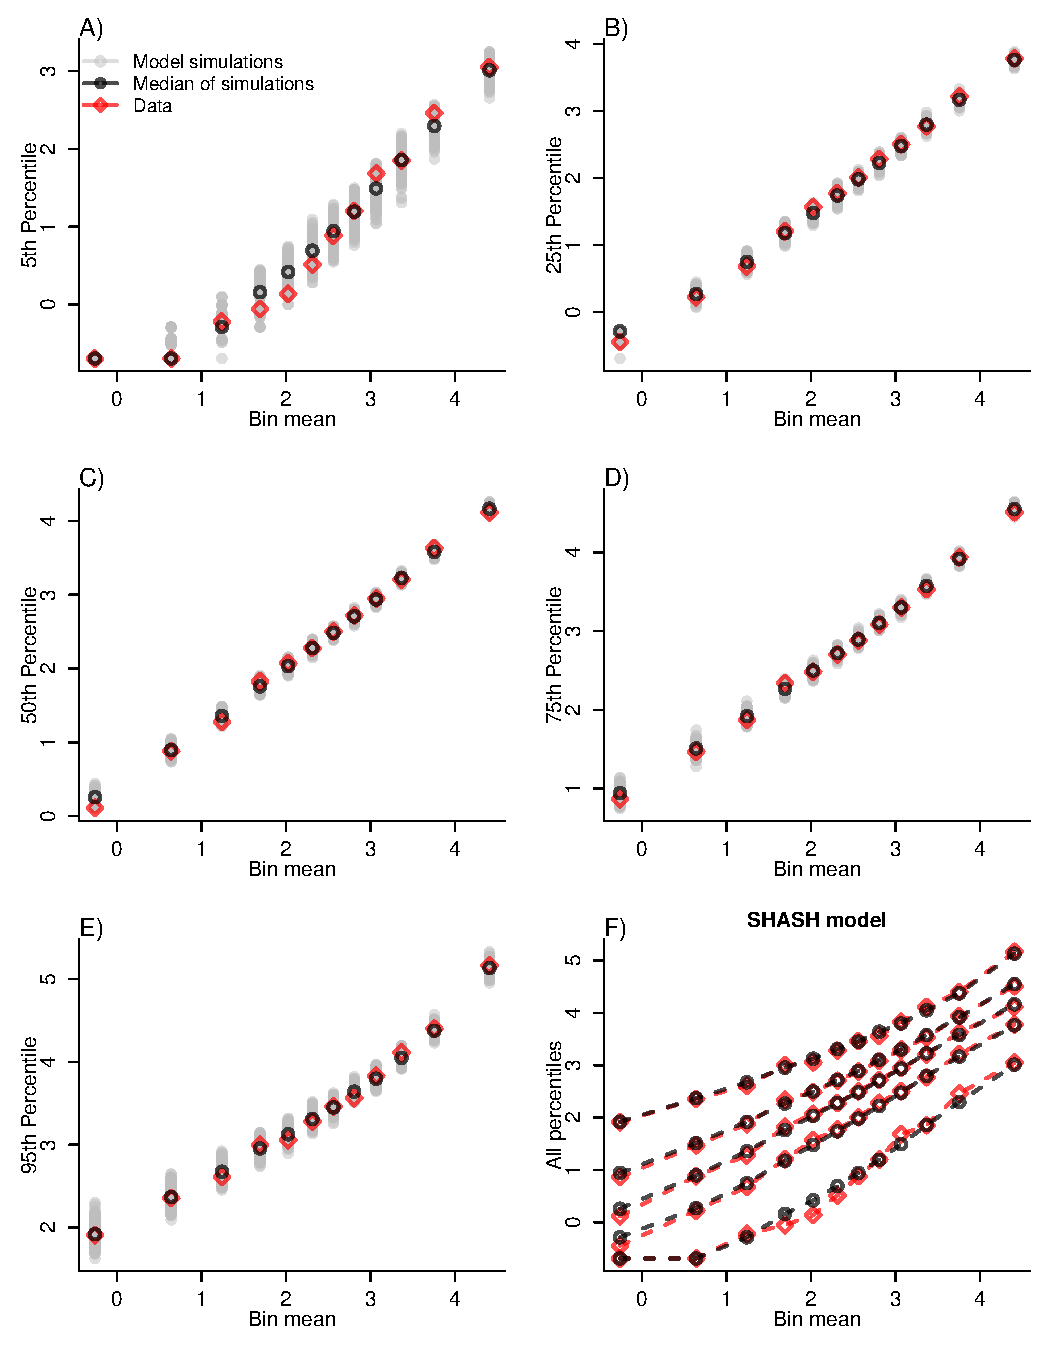
\includegraphics[width=.9\textwidth]{figures/QuantileComparePlotPSSP.pdf}
\caption{Binned data comparison of distribution quantiles between simulations of the fitted SHASH model (grey, black) and the actual data (red) for 
{P. spicata}. Individuals were binned based on their initial size. }
\label{fig:BinnedConditionalQuantiles}
\end{figure} 


\begin{figure}[tbp]
\centering
% 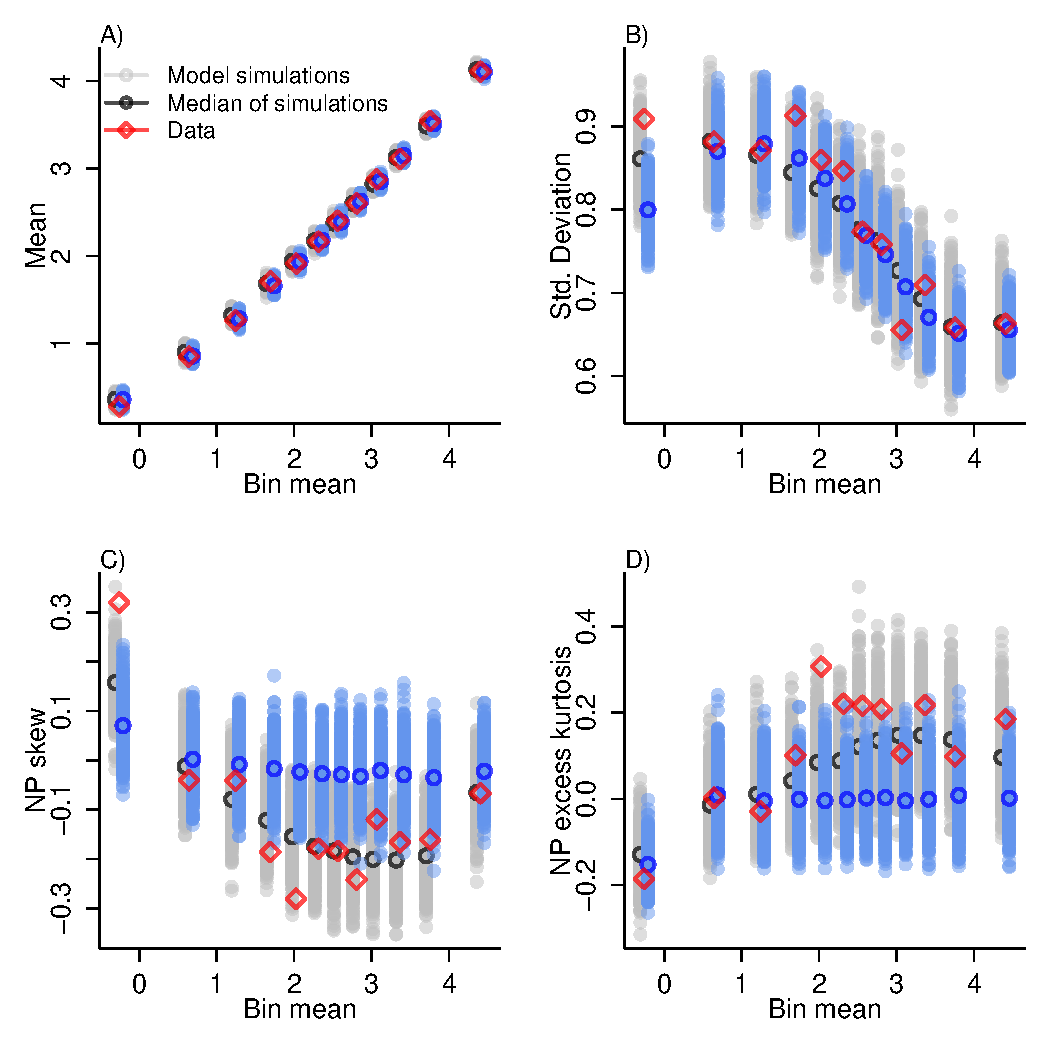
\includegraphics[width=.9\textwidth]{figures/MomentsComparePlotPSSP.pdf}
\caption{Binned data comparison of moments between simulations of the fitted SHASH model (grey, black) and the actual data (red) for 
{P. spicata}. Individuals were binned based on their initial size. }
\label{fig:BinnedConditionalMoments}
\end{figure} 

\item The model is easy to fit by ML. Does it do a good job of fitting the data? The comparison based on binned quantiles 
(fig. \ref{fig:BinnedConditionalQuantiles} looks pretty good except that the variation in the 5th percentile of the data
is more wiggly than the 5th percentile of the model. To eliminate this imperfection, we could perhaps try higher-order polynomials
for $\nu$ or $\tau$. 

\item More importantly, the SHASH model is a substantial improvement over the pilot Gaussian model, as seen in the
binned moments diagnostic plot, fig.  \ref{fig:BinnedConditionalMoments}. The fits to mean and standard deviation are
about as good, but only the SHASH model captures the skew and kurtosis and how they vary with size. 

\begin{figure}[tbp]
\centering
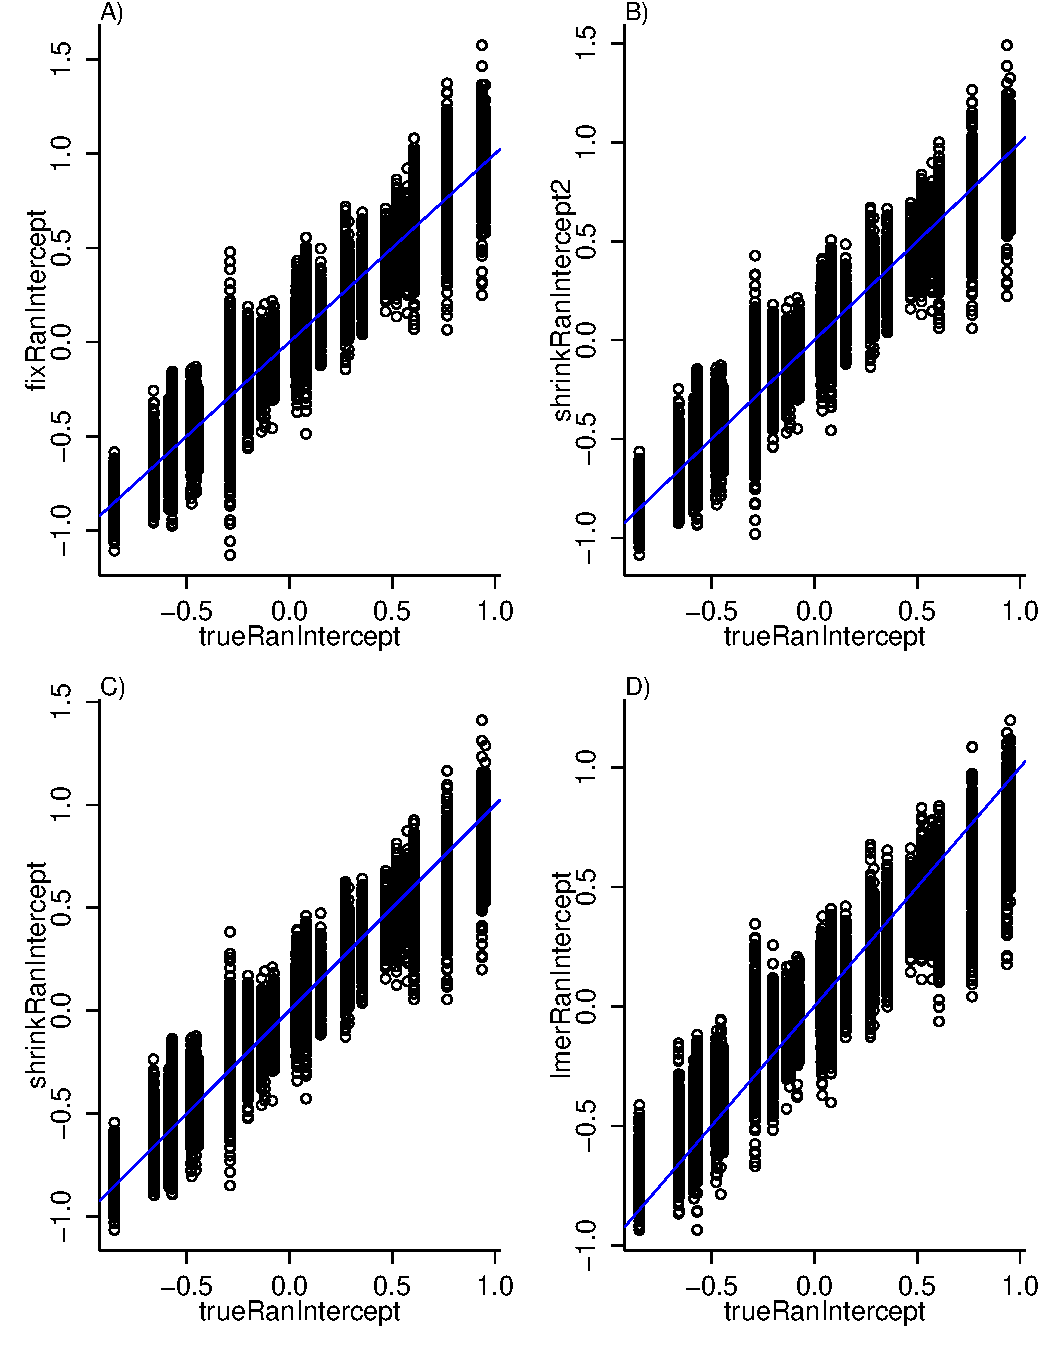
\includegraphics[width=.9\textwidth]{figures/PSSPShrinkageTest.pdf}
\caption{Comparison of ``true'' and estimated intercept year effects for {P. spicata}. }
\label{fig:ShrinkageTest}
\end{figure} 

\item Finally, a simulation study was done to see how well the shrinkage approach recovers known year effects. Fig. \ref{fig:ShrinkageTest}
illustrates the results for the intercept coefficient. Panels A,B,C,D are the fixed-effects estimates, recommended shrunk estimates,
more strongly shrunk estimates, and estimates from \texttt{lmer} using the fitted standard deviation from the pilot Gaussian model. 
Except for \texttt{lmer} they all look very similar, and they are. The recommended shrunk estimates had the lowest 
mean-square error for both slope and intercept (averaged across all years), and their sample variance was closest to the across-year 
variance in the data-generating model, but the improvement over the fixed-effects estimates was small: 

Intercept: true SD =  0.497, fixed SD =  0.516, shrunk SD = 0.468, lmer SD =  0.418 \\
Slope: True SD =  0.129, fixed SD = 0.137, shrunk SD = 0.126,  lmer SD = 0.106
 
Note that for both slope and intercept, the \texttt{lmer} estimates were over-smoothed (they under-estimated the
actual between-year variance). 

This study aligns with our earlier finding for IPMs with temporal random effects \citep{metcalf-etal-2015}: the simplest method (fitting as
fixed effects) works about as well as anything else. In that study shrinkage was not helpful at all, except that the fixed-effects 
and shrunk estimates were biased in opposite directions and therefore were useful as bounds on the truth. Here, shrinkage 
makes a small improvment. However, the biggest improvement in random effects estimation 
comes from using a better, non-Gaussian model for the growth distribution.  

\end{enumerate} 


\clearpage 

\section{Case study: creosote bush, \emph{Larrea tridentata}}
Our final case study comes from another perennial plant, the woody shrub \emph{Larrea tridentata}, whose dynamics we are studying at the Sevilleta LTER. 
At this site as elsewhere in the Southwest US, creosote bush is invading and displacing desert grassland habitats \citep{}.
The data described here were collected to understand patterns of density dependence in creosote bush demography, asking whether vital rates are maximized approaching zero density, at the leading edge of the expansion front (consistent with a `pulled' invasion), or whether there is a demographic advantage for shrubs at higher densities due to positive feedbacks expected for some ecosystem engineers (leading to a `pushed' invasion). 
We step through the growth analysis following our suggested workflow and then connect the growth model to a spatial inetgral projection (SIPM)  model that allows us to ask how `improved' growth modeling changes predictions for the speed of creosotebush encroachment (T. Drees, B. Ochocki, S. Collins, T. Miller, \textit{ms in prep}). 
The key features of this growth analysis are: initial size-dependence 

\subsection{A pilot Gaussian model}


\section{Discussion}

Here are some of the issues to be discussed.
\begin{itemize}
\item{Modeling the mean with gam vs glm}
\item{Modeling variance and higher moments as functions of covariates vs fitted values}
\item{Choosing a better distribution -- how to make the choice}
\item{Comparison of our method with beta regression}
\item{We have emphasize growth but same principles apply to other continuous state transitions, eg disease IPMs.}

\end{itemize}

\section*{Acknowledgements} 
This research was supported by US NSF grants DEB-1933497 (SPE) and .... 

\section{Authorship statement} 
All authors discussed all aspects of the research and contributed to developing methods, analyzing data, and writing and revising the paper.  

\section{Data accessibility statement}
No original data appear in this paper. Should the paper be accepted, all computer scripts supporting the results will be archived in a Zenodo package, with the DOI included at the end of the article. 
During peer review, our data and code are available at \url{https://github.com/texmiller/IPM_size_transitions}. 
	
\newpage 

%\bibliographystyle{EcologyLetters}
\bibliographystyle{apalike}
\bibliography{BetterGrowthModeling}

% ######################## Appendices ##############################
\newpage 
\clearpage 
% \setcounter{page}{1}
\setcounter{equation}{0}
\setcounter{figure}{0}
\setcounter{section}{0}
\setcounter{table}{0}
\setcounter{Box}{0}
\renewcommand{\theequation}{S.\arabic{equation}}
\renewcommand{\thetable}{S-\arabic{table}}
\renewcommand{\thefigure}{S-\arabic{figure}}
\renewcommand{\theBox}{S-\arabic{Box}}
\renewcommand{\thesection}{S.\arabic{section}}

\centerline{\Large{\textbf{Appendices}}}

\section{The Jones-Pewsey distribution} 
\citet{jones-pewsey-2009} introduced a simple, tractable generalization of the Normal distribution with two additional parameters determining  
asymmetry (skewness), and tail weight (kurtosis) which can be either lighter or heavier than the Gaussian. It is defined as a transformation
of a Normal(0,1) random variable usingthe hyperbolic sine function (sinh) and its inverse (asinh), as follows. The distribution family's base probability density  
$f_{\epsilon,\delta}$  is the probability density of the random variable $X_{\epsilon,\delta}$ where  
\be
Z = \sinh (\delta \; \mbox{asinh}(X_{\epsilon,\delta}) - \epsilon)
\label{eqn:JP1}
\ee
and $Z$ has a Normal(0,1) distribution.  Equivalently, 
\be
X_{\epsilon,\delta} = \sinh \left( \frac{1}{\delta} \; \mbox{asinh}(Z) + \frac{\epsilon}{\delta}\right).
\label{eqn:JP2}
\ee
Parameters $\delta=1, \epsilon=0$ give the Normal(0,1) distribution. Skewness has the sign of $\epsilon$, and
$\delta > 0$ controls tail weight, with heavier than Gaussian tails for $\delta<1$ and lighter than Gaussian tails for $\delta > 1$. 
A formula for the density $f_{\epsilon,\delta}$ is given by \citet[][eqn. 2]{jones-pewsey-2009}. 
The general four-parameter family with location parameter $\mu$ and scale parameter $\sigma$ is defined as the probability densities 
of $\mu + \sigma X_{\epsilon, \delta}$. We refer to this as the JP distribution family. 

As is unfortunately the case for most four-parameter distributions $\mu$ is not the mean, $\sigma$ is not the standard deviation, $\epsilon$ is not
the skew and $\delta$ is not the kurtosis. All else being equal, larger $\mu$  gives a larger mean, larger $\sigma$ gives a higher
standard deviation, higher $\epsilon$ gives higher asymmetry, and higher $\delta$ gives heavier tail weight.  But each moment is jointly determined 
by all four parameters. 

The main advantage of the JP distribution is that the attainable combinations of skewness and kurtosis are very broad, compared to other 
four-parameter families, and come very close to the theoretical limits on kurtosis as a function of skewness \citep[][Fig.  2]{jones-pewsey-2009}. 
Additionally, being a transformation of the Normal makes it very simple to generate random numbers from the distribution, and to compute 
probability density, cumultive distribution, and quantile functions. There are also simple analytic formulas for the first four moments
\citep[][p. 764]{jones-pewsey-2009} which we use below to define a centered and scaled version in which $\mu$ and $\sigma$ 
are the mean and standard deviation. 

The definition \eqref{eqn:JP2} shows that the distribution depends on $\epsilon$ only through the ratio $\epsilon/\delta$. We have found
that this property can be problematic for estimating distribution parameters. Even with good sized ($n=250$ or 500) data sets generated from the 
distribution with known parameters, both maximum likelihood and Bayesian estimation were unstable for some values of $\epsilon$ and $\delta$, 
occasionally yielding estimates far from the truth. One cause was a ridge in the $(\epsilon,\delta)$ likelihood surface with a constant of 
$\epsilon/\delta$. Another is that when $\delta$ is large,  changes in $\epsilon$ have little effect. 

To avoid that problems, we reparameterize the distribution as follows: 
\be
X_{\lambda,\tau} = \sinh \left( e^{-\tau} \; \mbox{asinh}(Z) + \lambda \right).
\label{eqn:SJP}
\ee
Thus, the two parameterizations are related by
\be
\delta = e^{\tau}, \epsilon= \delta \lambda =  e^{\tau} \lambda.
\ee
The definition of $\tau$ allows it to take any real value, with negative values giving thinner than Gaussian tails and positive
values giving fatter than Gaussian tails. $\lambda$ also can take any real value, and the distribution's skew has the same sign as $\lambda$. 
Because the $\sinh$ function is nonlinear, it is still the case that the skew depends on $\tau$ as well as $\lambda$, but the
``crosstalk'' between the kurtosis and skew parameters is weaker. As  a result, we found that maximum likelihood estimation of parameter values was 
generally more reliable if the distribution is parameterized in terms of $\tau$ and $\lambda$. 

\section{Estimating mixed-effects models using shrinkage}

Ecologists often fit demographic and other statistical models that include random effects terms to
quantify variation among years, spatial locations, individuals, etc. Random effects
are a natural choice when interest centers on the magnitude of variation (e.g., how much does mortality vary among years?)  
rather than individual values (e.g., mortality in 2013). They also allow each estimate to 
``borrows strength'' from others, so that (for example) the estimate from a year with small sample size (and thus large 
sampling variability) is shifted towards the center of the overall distribution. 

Specialized software is often used to fit such models, such as the \textbf{nlme, lme4, mgcv} and \textbf{gamm4} libraries in R,  
but these only allow a small subset of the distribution families we want to consider for modeling growth increments (the \textbf{gamlss} 
package allows many distribution families, but in our experience, even when random effects are simple in structure 
the fitting algorithms often fail to converge or fail to find the global optimum). 

One way past this limitation is Bayesian estimation, using STAN with user-written (or borrowed) 
code for the chosen growth distribution (see section XX for an example). 
In this appendix we describe another option, introduced by \citet{link-nichols-1994} and \citet{gould-nichols-1998}: 
fitting a fixed-effects model by Maximum Likleihood, followed by shrinkage of coefficient estimates. 
None of the ideas here are original. The material overlaps Appendix S1 of \citet{metcalf-etal-2015}, 
but for completeness we make it self-contained. Appendix D of \citet{cooch-white-2020} (written by K.D. Burnham)
provides more details and examples in the context of capture-recapture analysis. 

Here we explain shrinkage using a simple model based on our analysis of \emph{Pseudoroegneria spicata}. 
That model includes random effects for between-year variation in the slope and intercept of future size 
(log area) as a function of initial size. To keep the example simple, we assume that initial size 
and year are the only covariates, and we assume that growth increments 
follow a skew-Normal distribution with nonconstant variance and constant skew parameter. 
Code for this example is in the script \texttt{SimpleShrinkageExample.R}. The first part of the script generates
an artificial data set by fitting the model to a subset of the growth data (20th century Control plots), and
randomly generating new ``size next year'' values for each individual in the actual data set. 
The second part contains the ``data'' analysis. 

As in our \emph{P. spicata} analysis, we assumed that that the skew and kurtosis parameters were functions
of the location parameter; this dominated $(\Delta AIC \approx 30)$ the alternate 
model with skew and kurtosis depending on initial size.   
The analogous Gaussian model, with constant variance, could be fitted as follows using \texttt{lmer}:
\begin{lstlisting}
lmer(new.size ~ init.size + (init.size|year), data=growthData, REML=TRUE); 
\end{lstlisting}
where \texttt{growthData} is a data frame holding the data with \texttt{year} as an unordered factor. For our skew-Normal
model, we instead use maximum likelihood with all between-year variation included as fixed effects. The appropriate design
matrix is easily constructed using the \texttt{model.matrix} function: 
\begin{lstlisting}
U = model.matrix(~year + init.size:year - 1, data=growthData)
\end{lstlisting}
If there are $T$ years, the matrix \texttt{U} specified in this way has $2T$ columns corresponding to $n$ annual 
intercepts and $T$ annual slopes. 

Using this design matrix, we can readily write a log likelihood function for use with 
the \textbf{maxLik} package, with a log link function for the variance because it is necessarily positive: 
\begin{lstlisting}
LogLik=function(pars,new.size,U){
    pars1 = pars[1:ncol(U)]; pars2=pars[-(1:ncol(U))];
    mu = U%*%pars1;  
    sigma = exp(pars2[1]+pars2[2]*mu);
    dSN1(new.size, mu=mu, sigma=sigma, nu=pars2[3], log=TRUE)
}
\end{lstlisting} 

Parameters and their standard errors can then be estimated with \texttt{maxLik}, 
starting from a random guess: 
\begin{lstlisting}
start=c(runif(ncol(U)), rep(0,3))
out=maxLik(logLik=LogLik,start=start, new.size=simData$new.size,U=U,
  method="BHHH",control=list(iterlim=5000,printLevel=1),finalHessian=TRUE);
coefs = out$estimate; # parameters
V = vcov(out); SEs = sqrt(diag(V));	# standard errors 
\end{lstlisting}  
In real life we would repeat the optimization several times with several different starting values, to be confident that
the optimal parameter values had been found. 

Focus now on the year-specific intercept parameters $\hat{a}_t, t = 1,2,\cdots T$. 
We can view the year-specific estimates $\hat{a}_t$ as consisting of unobserved true values $a_t$ plus sampling error:
\be
\hat{a}_t= a_t + \varepsilon_t 
\ee
Because of the sampling errors, the sample variance of
the estimates $\hat{a}_t$ is an upward-biased estimate of the true across-year variance in the parameter. 
That is undesirable if the model will be used to project how temporal variability affects population dynamics. 
However, maximum liklihood estimation gives us an approximaten variance-covariance matrix $\hat{V}$ of the
sampling errors, \texttt{V} in the code above. With that information, we can estimate the parameters
of a random effects model for the intercept parameters, and thereby improve the year-specific estimates and
the estimate of the across-year variance.  

The model is as follows. We make the standard mixed-models assumptions that the $a_t$ are drawn 
independently from some fixed distribution with unknown variance $\sigma^2$. We also assume that the estimates 
$\hat{a}_t$ are unbiased, that is
\be
\mathbb{E}(\varepsilon_t \vert a_t) = 0.    
\ee
These are optimistic assumptions, but not excessively optimistic. Some degree of temporal correlation will often be
present, and as we explain at the end, it is theoretically possible to account for it. 
Maximum likelihood parameter estimates are not unbiased, but if the assumptions
of maximum likelihood are satisfied the bias is asympototically negligible compared to the standard error (the 
bias scales as the inverse of sample size, the standard error as the square root of the inverse of sample size).  

Let $S^2$ denote the sample variance of the estimates $\hat{a}_t$. It can then be shown that 
\be
\mathbb{E}(S^2) = \sigma^2  + \frac{1}{T}\sum\limits_{t=1}^T \mathbb{E} Var(\varepsilon_t) 
- \frac{1}{T(T-1)}\sum\limits_{i=1}^{j-1} \sum\limits_{j=1}^T \mathbb{E}Cov(\varepsilon_i, \varepsilon_j). 
\label{eqn:biasTerms}
\ee
This is eqn. (1) in \citet{gould-nichols-1998} in our notation, without the term that 
results from temporal autocorrelation. 

The terms besides $\sigma^2$ on the right-hand are the expected impact of sampling error on the across-year variance
of the parameter estimates; their presence makes $S^2$ a biased estimated of $\sigma^2$. However,
all of those terms correspond to entries in the variance-covariance matrix $V$. We can therefore use our estimated
variance-covariance matrix $\hat{V}$ to removes the bias due to sampling variability: 
\be
\hat{\sigma^2}  = S^2 - \frac{1}{T}\sum\limits_{t=1}^T \hat{V}_{t,t} + 
\frac{1}{T(T-1)}\sum\limits_{i=1}^{j-1} \sum\limits_{j=1}^T \hat{V}_{i,j}. 
\label{eqn:hatSigma}
\ee
$\hat{\sigma^2}$ estimates the variance of the distribution from which the $a_t$ are assumed
to be drawn. 

Using that estimate, we can adjust the year-specific estimates to reduce the expected 
impact of sampling error. Depending on your purposes, there are two possible adjustments. 
The first option is the one used in the popular capture-recapture analysis 
software Mark \citet{cooch-white-2020}, 
\be
\widetilde{a}_t = \bar{\hat{a_t}} + \sqrt{\frac{\hat{\sigma}^2}{\hat{\sigma}^2 + \hat{V}_{t,t}}}\left (\hat{a_t} - \bar{\hat{a_t}} \right). 
\label{eqn:ShrinkLess}
\ee
The name ``shrinkage'' comes from the fact that each estimate is adjusted towards the overall mean, with 
larger adjustments of values that have higher estimated sampling error variance, $\hat{V}_{t,t}$. 
This shrinkage estimate has the property that the expected sample variance of the 
adjusted estimates $\widetilde{a}_t$ is very close to $\hat{\sigma^2}$, so the $\widetilde{a}_t$ approximate
the actual amount of parameter variation. 

The second is to replace $\hat{a}_t$ by the least-squares estimate of $a_t$ under the 
additional assumption that the $a_t$ are drawn from a Gaussian distribution; this is given by 
\be
\widetilde{a}_t = \bar{\hat{a_t}} + \frac{\hat{\sigma}^2}{\hat{\sigma}^2 + \hat{V}_{t,t}}\left (\hat{a_t} - \bar{\hat{a_t}} \right). 
\label{eqn:ShrinkMore}
\ee
This option is theoretically preferable if the Gaussian assumption is reasonable, and you are more interested in year-specific values rather 
than across-year variance. However, \citet{metcalf-etal-2015} found that even \eqref{eqn:ShrinkLess}, which does 
less shrinkage, resulted in a small downward bias in the temporal variance of population growth rates. This argues for  
always using the first option, and we do the same here. 

We differ from MARK, however, in using \eqref{eqn:hatSigma} rather than an iterative method that takes \eqref{eqn:hatSigma} as its 
starting estimate and refines the estimate by using weighted least squares based on the current estimate. 
\citet{metcalf-etal-2015} found, in simulation studies, that the iterative method was either slightly beneficial 
or wildly inaccurate. We therefore advise against it. 

Finally, as mentioned above, the estimate of $\sigma^2$ can account for temporal autocorrelation in the $a_t$. 
When present, those correlations add a term to eqn. \eqref{eqn:biasTerms} (see eqn. (1) in \citet{gould-nichols-1998}), 
which can be estimated from the sample autocorrelation of the $\hat{a}_t$. We do not recommend doing this (and therefore omit
the formulas) because the autocorrelations can only be reliably estimated if they fall to nearly zero within lag $m \ll T$, in which
case the autocorrelation term is small (specifically, $O(m/T)$). Otherwise, the random error from using poorly estimated 
autocorrelations is likely to outweight the small bias from omitting that term. 

The take-home message is that estimating random effects from the regression coefficients is very simple: 
\begin{lstlisting}
# Variance-covariance matrices for intercepts and slopes
V1 = V[1:T,1:T]; V2 = V[(T+1):(2*T),(T+1):(2*T)]; 
# Extract year-specific intercepts, center them to zero   
fixed.fx = coefs[1:T]; fixed.fx = fixed.fx-mean(fixed.fx); 

# Estimate sigma^2
var.hat = mean(fixed.fx^2) - mean(diag(V1)) + 
              (sum(V1)-sum(diag(V1)))/(2*T*(T-1)); 

# Shrink deviations from the mean 
shrinkRanIntercept = fixed.fx*sqrt(var.hat/(var.hat + diag(V1)));

# Do it all again for the slopes 
fixed.fx2 = coefs[(T+1):(2*T)]; fixed.fx2 = fixed.fx2-mean(fixed.fx2); 
var2.hat = mean(fixed.fx2^2) - mean(diag(V2)) + 
               (sum(V2)-sum(diag(V2)))/(2*T*(T-1)); 
shrinkRanSlope = fixed.fx2*sqrt(var2.hat/(var2.hat + diag(V2))); 
\end{lstlisting}

The figure below shows the results for one artificial PSSP ``data'' set, having $T=22$ years and growth measurments on 
about 175 individuals/year on average. The true random year effects (the ones used to generate the data) are recovered
with good accuracy and no bias. In particular there is no sign of extreme values being pulled in too far
towards the mean, which would cause an S-shaped graph of estimated versus true values. 

\bigskip 

\centerline{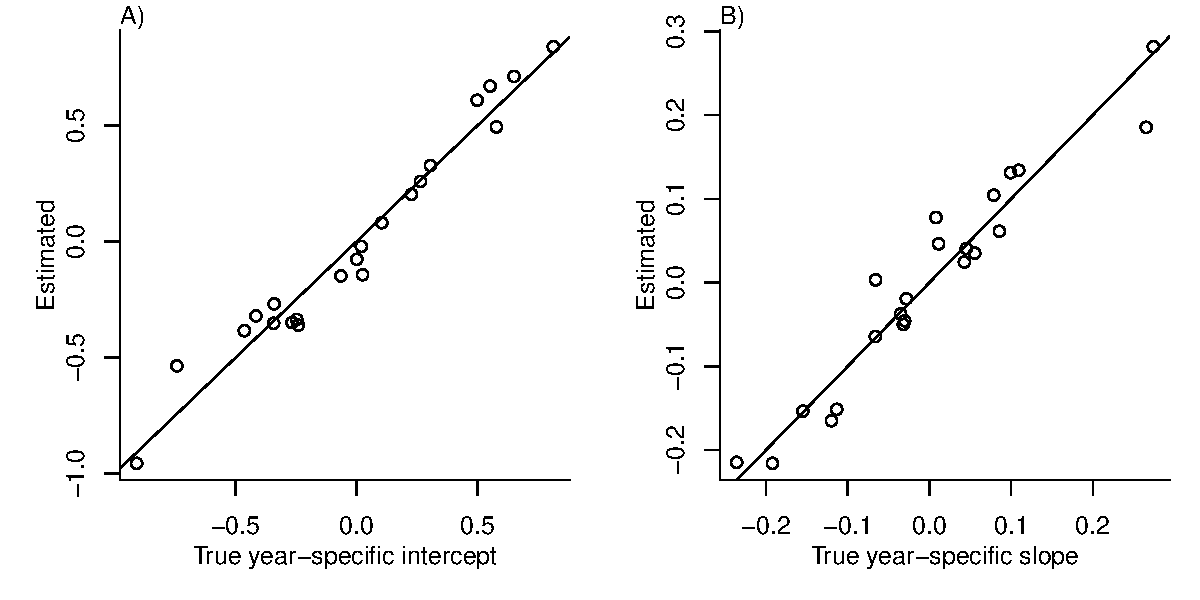
\includegraphics[width=\textwidth]{figures/SimpleShrinkage.pdf}}

  
\end{document}